\documentclass[cn,10pt,math=newtx,chinesefont=founder,device=ig]{elegantbook}

\title{高中物理科教師甄試詳解}
\subtitle{2019年}

\author{李宥頡}
\institute{National Taiwan University}
%\date{May 2, 2021}
%\version{4.1}
%\bioinfo{自定义}{信息}

%\extrainfo{寶寶肚子餓—— 顏利蓁}

\setcounter{tocdepth}{3}

%\logo{logo-blue.png}
%\cover{cover.jpg}

% 本文档命令
\usepackage{array}
\newcommand{\ccr}[1]{\makecell{{\color{#1}\rule{1cm}{1cm}}}}

\definecolor{customcolor}{RGB}{32,178,170}
\colorlet{coverlinecolor}{customcolor}



\begin{document}

\maketitle
\frontmatter

\chapter*{序}



\tableofcontents

\mainmatter

\chapter{台中女中}


\section{填充題}

\begin{example}
  如圖所示,兩上下底面平行的長方體木塊A、B重疊在一起,置於傾角為$\theta$的固定斜面上,木塊A、B的質量分別為$m_A, m_B$,
  A與斜面間的動摩擦係數為$\mu_1$,B與A之間的靜摩擦係數為$\mu_2$,已知兩木塊都從靜止開始滑下,且A、B之間始終相對靜止,
  則木塊B受到的摩擦力應為? (重力加速度以g表示)\\
  \rightline{[台中女中教甄109]}
\end{example}
\begin{solution}
$m_{B}g\cos \theta \mu_1$
\end{solution}
\begin{note}
  相對靜止:代表物體所受摩擦力為靜摩擦力
\end{note}
\begin{figure}[htbp]
  \flushright
  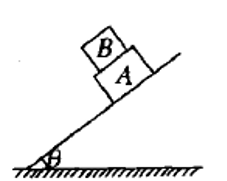
\includegraphics[width=0.2\textwidth]{109中女1.png}
\end{figure}
\newpage

\begin{example}
  人和雪橇的總質量為75kg,沿傾角$\theta=37^\circ $且足夠長的斜坡向下滑動。已知所受的空氣阻力與速度成正比,比例常數$k$未知,
  從某時刻開始計時,測得雪橇運動的速度對時間($v-t$)關係圖如右圖中的曲線AD所示,圖中AB是曲線在A點的切線,切線上一點B的坐標為(4,15),
  CD是曲線AD的漸近線。若重力加速度$g=10m/s^2$,試求雪橇與斜坡間的動摩擦係數應為何?\\
  \rightline{[台中女中教甄109]}
\end{example}
\begin{solution}
  $\frac{1}{8}$
\end{solution}
\begin{figure}[htbp]
  \flushright
  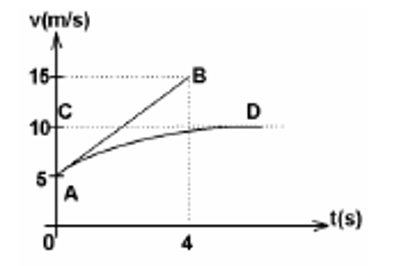
\includegraphics[width=0.3\textwidth]{109中女2.png}
\end{figure}
\newpage
%%%%%%%%%%%%%%%%%%%%%%%%%%%%%%%%%%%%%%%%%%%%%%%%%%%%%%%%%%%%%%%%%%%%%%%%%%%%%%%%%%%%
\begin{example}
  如右圖所示,光滑平行金屬軌的ab部分是平滑的曲線,該處沒有磁場。bc、cd的部分置於水平桌面上,該處有均勻鉛直向上的磁場B,且bc部分的寬度2L是cd部分的兩倍。今有兩相同材質的導體棒P、Q,
  質量分別為m、2m,Q原靜置於cd部分,P則由高出桌面h處,由靜止滑下,設bc、cd 的長度均甚長,且P、Q 最後分別於bc和cd上作等速度運動,則導體棒P的終端速率應為?\\
  \rightline{[台中女中教甄109]}
\end{example}

\begin{solution}
  $\frac{\sqrt{2gh}}{9}$
\end{solution}

\begin{figure}[htbp]
  \flushright
  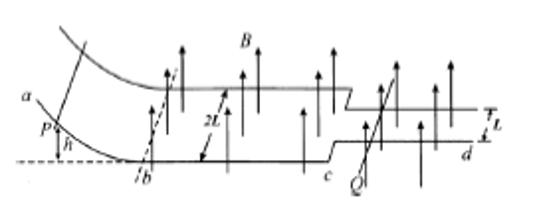
\includegraphics[width=0.4\textwidth]{109中女3.png}
\end{figure}
\newpage
%%%%%%%%%%%%%%%%%%%%%%%%%%%%%%%%%%%%%%%%%%%%%%%%%%%%%%%%%%%%%%%%%%%%%%%%%%%%%%%%%%%%
%%%%%%%%%%%%%%%%%%%%%%%%%%%%%%%%%%%%%%%%%%%%%%%%%%%%%%%%%%%%%%%%%%%%%%%%%%%%%%%%%%%%
\begin{example}
  一道單色光線自空氣射入液體中,遇到平面鏡M再反射到液面,若液體對空氣的折射率為$\sqrt{2}$,
  而在A點的入射角為$45^\circ$,則右圖中$\theta$大於等於\_\_\_\_\_\_\_,才會在B點引起全反射。\\
  \rightline{[台中女中教甄109]} 
\end{example}
\begin{solution}
  $7.5^\circ$
\end{solution}
\begin{figure}[htbp]
  \flushright
  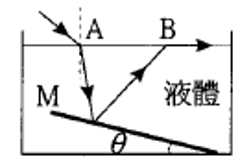
\includegraphics[width=0.3\textwidth]{109中女4.png}
\end{figure}
\newpage
\begin{example}
  A、B兩木塊原先處於靜止的狀態,已知A、B兩木塊的質量比為2:1可忽略滑輪組與繩索的質量與所有摩擦力。已知重力加速度為g,求放手之後B的加速度為何?\\
  \rightline{[台中女中教甄109]}
\end{example}
\begin{solution}
  $\frac{2g}{11}$
\end{solution}
\begin{figure}[htbp]
  \flushright
  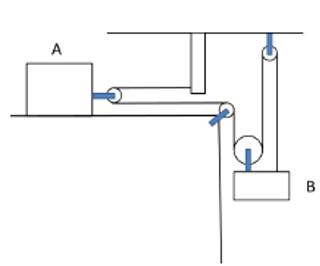
\includegraphics[width=0.3\textwidth]{109中女5.png}
\end{figure}
\newpage
%%%%%%%%%%%%%%%%%%%%%%%%%%%%%%%%%%%%%%%%%%%%%%%%%%%%%%%%%%%%%%%%%%%%%%%%%%%%%%%%%%%%
%%%%%%%%%%%%%%%%%%%%%%%%%%%%%%%%%%%%%%%%%%%%%%%%%%%%%%%%%%%%%%%%%%%%%%%%%%%%%%%%%%%%
\begin{example}
  我們可利用用文氏管測量氣體的壓力差,現有一口徑不同的管子,內部有氣體穩定的通過,如圖所示。已知A、B兩點所在橫截面的面積比為2:1,且氣流通過A點的速率為$v_0$。
  氣體密度為$d$,水銀密度為$d^\prime$,A、B兩點下方水銀柱高度分別為$h_a$、$h_b$,則$h_=b-h_a$為何?(以$d, d^\prime, v_0$表示)\\
  \rightline{[台中女中教甄109]}
\end{example}
\begin{solution}
  $\frac{3dv_{0}^{2}}{2d^\prime g}$
\end{solution}
\begin{figure}[htbp]
  \flushright
  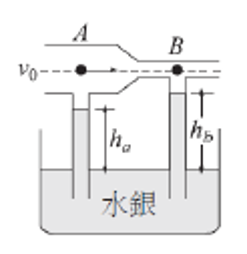
\includegraphics[width=0.25\textwidth]{109中女6.png}
\end{figure}
\newpage
%%%%%%%%%%%%%%%%%%%%%%%%%%%%%%%%%%%%%%%%%%%%%%%%%%%%%%%%%%%%%%%%%%%%%%%%%%%%%%%%%%%%
\begin{example}
  如附圖之線路,不計導線電阻及電池內電阻,平行板電容為2.0 pF(1 pF=$1\times 10^{-12}F$),兩板間距為2.0 mm,充電完畢後,
  求平行板電容器內的正電板的電量為\_\_\_(1)\_\_\_庫侖,平行板間的電場為\_\_\_(2)\_\_\_V/m\\
  \rightline{[台中女中教甄109]}
\end{example}
\begin{solution}
  (1)$8\times 10^{-12}$\ \ (2)$2\times 10^3$
\end{solution}
\begin{figure}[htbp]
  \flushright
  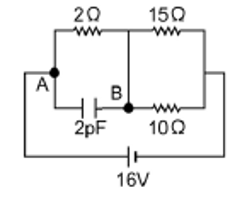
\includegraphics[width=0.3\textwidth]{109中女7.png}
\end{figure}
\newpage
%%%%%%%%%%%%%%%%%%%%%%%%%%%%%%%%%%%%%%%%%%%%%%%%%%%%%%%%%%%%%%%%%%%%%%%%%%%%%%%%%%%%
\begin{example}
  右圖是把量程為3毫安培的安培計改裝成歐姆計的結構示意圖,其中串接的電池電動勢=1.5伏特(無內電阻),
  經改裝後,若將原電流計3毫安培刻度處的刻度值定為零歐姆位置,則2毫安培刻度處應標\_\_\_\_\_\_\_歐姆\\
  \rightline{[台中女中教甄109]} 
\end{example}
\begin{solution}
  250
\end{solution}
\begin{figure}[htbp]
  \flushright
  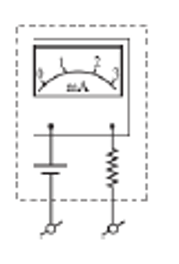
\includegraphics[width=0.2\textwidth]{109中女8.png}
\end{figure}
\newpage
%%%%%%%%%%%%%%%%%%%%%%%%%%%%%%%%%%%%%%%%%%%%%%%%%%%%%%%%%%%%%%%%%%%%%%%%%%%%%%%%%%%%
%%%%%%%%%%%%%%%%%%%%%%%%%%%%%%%%%%%%%%%%%%%%%%%%%%%%%%%%%%%%%%%%%%%%%%%%%%%%%%%%%%%%
\begin{example}
  質量為m的小球被兩個彈性係數為k的相同輕質彈簧繫在一個質量為M的盒子中(如圖所示),
  盒從高h處靜止釋放(自桌面量起),在盒子釋放瞬間,兩彈簧均未發生形變,且小球相對盒靜止。
  若盒與桌面在發生完全非彈性碰撞後還能跳起來,則釋放高度h至少為何?
  (設小球只能在鉛直方向運動, 重力加速度以g表示)\\ 
  \rightline{[台中女中教甄109]} 
\end{example}
\begin{solution}
  $\frac{Mg}{2k}+\frac{M^2 g}{4mk}$
\end{solution}
\begin{figure}[htbp]
  \flushright
  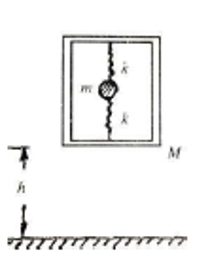
\includegraphics[width=0.3\textwidth]{109中女9.png}
\end{figure}
\newpage
%%%%%%%%%%%%%%%%%%%%%%%%%%%%%%%%%%%%%%%%%%%%%%%%%%%%%%%%%%%%%%%%%%%%%%%%%%%%%%%%%%%%

%%%%%%%%%%%%%%%%%%%%%%%%%%%%%%%%%%%%%%%%%%%%%%%%%%%%%%%%%%%%%%%%%%%%%%%%%%%%%%%%%%%%
\begin{example}
  一個質量均勻分布的絕緣細圓環,其半徑為 R ,質量為 m 。
  令此絕緣環均勻帶正電,總電量為Q,現將此環平放在絕緣的光滑水平桌面上,
  並處於磁場強度為 B 的均勻磁場中,磁場的方向鉛直向下。當此環通過其中心的鉛直軸以等角速度$\omega$沿圖示方向旋轉時,
  此環上所產生的張力量值為?\\
  \rightline{[台中女中教甄109]} 
\end{example}
\begin{solution}
  $\frac{R\omega}{2\pi}(m\omega+BQ)$
\end{solution}
\begin{figure}[htbp]
  \flushright
  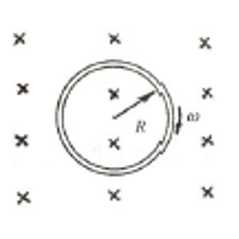
\includegraphics[width=0.25\textwidth]{109中女10.png}
\end{figure}
\newpage
%%%%%%%%%%%%%%%%%%%%%%%%%%%%%%%%%%%%%%%%%%%%%%%%%%%%%%%%%%%%%%%%%%%%%%%%%%%%%%%%%%%%
%%%%%%%%%%%%%%%%%%%%%%%%%%%%%%%%%%%%%%%%%%%%%%%%%%%%%%%%%%%%%%%%%%%%%%%%%%%%%%%%%%%%
\begin{example}
  圖所示的導熱良好的容器,中間有一個固定的隔板將其分為A、B兩室,
  已知兩室體積均為 V,且外界溫度為 T(絕對溫度)。今在A、B兩室分別裝入質量均為 M 克的氖及氦氣
 (氖的原子量為20,氦的原子量為4)試求:(已知理想氣體常數為R ) 
  \begin{enumerate}
    \item 氖的內能
    \item 若將隔板的固定器拆除,使其能自由運動。當隔板停止運動時,氦氣的體積
  \end{enumerate}
  
  \rightline{[台中女中教甄109]} 
\end{example}
\begin{solution}
  (1)$\frac{3}{40}MRT$ \ \ (2)$\frac{5V}{3}$
\end{solution}
\begin{figure}[htbp]
  \flushright
  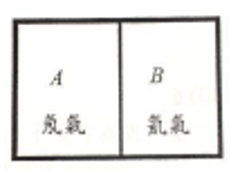
\includegraphics[width=0.2\textwidth]{109中女11.png}
\end{figure}
\newpage
%%%%%%%%%%%%%%%%%%%%%%%%%%%%%%%%%%%%%%%%%%%%%%%%%%%%%%%%%%%%%%%%%%%%%%%%%%%%%%%%%%%%

%%%%%%%%%%%%%%%%%%%%%%%%%%%%%%%%%%%%%%%%%%%%%%%%%%%%%%%%%%%%%%%%%%%%%%%%%%%%%%%%%%%%
\begin{example}
  取兩片玻璃相互貼近,如果兩片玻璃間夾入兩條相同且直徑在微米等級的細金屬線,
  當以波長為600 nm 的光線照射時,由上方無法看到光;當照射光線波長做連續調整至480 nm 時,
  由上方觀察恰好由暗轉為最亮光;則最可能的細金屬線直徑為\_\_\_\_\_\_\_ 微米\\
  \rightline{[台中女中教甄109]} 
\end{example}
\begin{solution}
  0.6
\end{solution}
\newpage
%%%%%%%%%%%%%%%%%%%%%%%%%%%%%%%%%%%%%%%%%%%%%%%%%%%%%%%%%%%%%%%%%%%%%%%%%%%%%%%%%%%%

%%%%%%%%%%%%%%%%%%%%%%%%%%%%%%%%%%%%%%%%%%%%%%%%%%%%%%%%%%%%%%%%%%%%%%%%%%%%%%%%%%%%
\begin{example}
  有一子彈型透鏡其材質為玻璃,其尺寸大小如圖所示,其折射率為1.5,其中一面是平面另一面為球面,
  而球面的曲率半徑是5.0cm,若有一物體置於透鏡平面左方10cm處,則最終成像於\_\_\_\_\_\_\_cm處
  (此位置請以O點為參考點,向右為正)\\
  \rightline{[台中女中教甄109]} 
\end{example}
\begin{solution}
  +25
\end{solution}
\begin{figure}[htbp]
  \flushright
  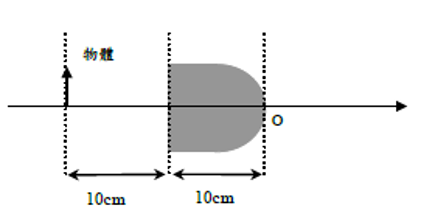
\includegraphics[width=0.3\textwidth]{109中女13.png}
\end{figure}
\newpage
%%%%%%%%%%%%%%%%%%%%%%%%%%%%%%%%%%%%%%%%%%%%%%%%%%%%%%%%%%%%%%%%%%%%%%%%%%%%%%%%%%%%

%%%%%%%%%%%%%%%%%%%%%%%%%%%%%%%%%%%%%%%%%%%%%%%%%%%%%%%%%%%%%%%%%%%%%%%%%%%%%%%%%%%%
\begin{example}
  質譜儀測定同位素時,質量數為39與41的鉀單價離子先在電場加速,
  接著進入垂直離子運動方向的均勻磁場中。在實驗過程中,加速電壓平均值為$V_0$,
  若因儀器不完善使電壓有微幅變化$\pm \Delta V$。欲使兩同位素束不發生覆蓋,則$\Delta V$/ 要小於\ \ \ \  \%。\\
  \rightline{[台中女中教甄109]} 
\end{example}
\begin{solution}
  2.5
\end{solution}
\begin{figure}[htbp]
  \flushright
  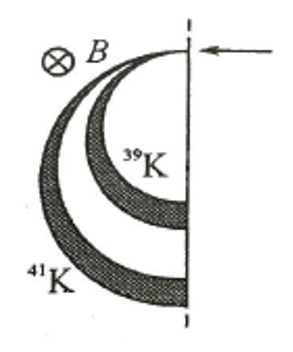
\includegraphics[width=0.3\textwidth]{109中女14.png}
\end{figure}
\newpage
%%%%%%%%%%%%%%%%%%%%%%%%%%%%%%%%%%%%%%%%%%%%%%%%%%%%%%%%%%%%%%%%%%%%%%%%%%%%%%%%%%%%
\begin{example}
  長度為$l$的輕桿在鉛直平面上並被固定在O點的光滑轉軸上,O將輕桿分為長度1:3的兩個部分,
  桿一端裝上質量為m的重球,桿另一端固定在彈力常數為k的水平彈簧上,當桿豎直時彈簧無形變。
  試求對小球作微小擾動時其振動週期為何?\\
  \rightline{[台中女中教甄109]} 
\end{example}
\begin{solution}
  $6\pi \sqrt{\frac{ml}{kl+12mg}}$
\end{solution}
\begin{figure}[htbp]
  \flushright
  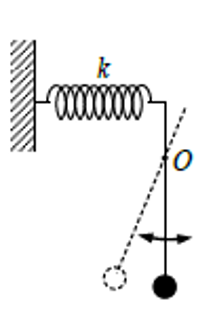
\includegraphics[width=0.2\textwidth]{109中女15.png}
\end{figure}
\newpage
%%%%%%%%%%%%%%%%%%%%%%%%%%%%%%%%%%%%%%%%%%%%%%%%%%%%%%%%%%%%%%%%%%%%%%%%%%%%%%%%%%%%



%%%%%%%%%%%%%%%%%%%%%%%%%%%%%%%%%%%%%%%%%%%%%%%%%%%%%%%%%%%%%%%%%%%%%%%%%%%%%%%%%%%%
\begin{example}
  如圖所示,半徑為2R與R的兩均勻圓盤,各自繞垂直於其盤面的中心軸以角速度$\omega$和$\omega$轉動,
  且兩轉軸互相平行。已知其對中心軸的轉動慣量分別為$4I$與$I$,若使兩圓盤以邊緣接觸,
  則兩盤邊緣因有摩擦力$f$的作用,最後達到穩定狀態。則從接觸到穩定狀態共歷時?\\
  \rightline{[台中女中教甄109]} 
\end{example}
\begin{solution}
  $\frac{I \omega}{2fR}$
\end{solution}
\begin{figure}[htbp]
  \flushright
  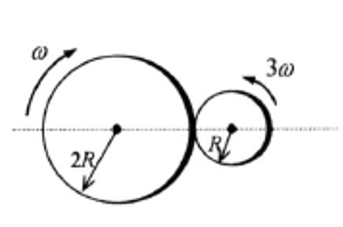
\includegraphics[width=0.3\textwidth]{109中女16.png}
\end{figure}
\newpage
%%%%%%%%%%%%%%%%%%%%%%%%%%%%%%%%%%%%%%%%%%%%%%%%%%%%%%%%%%%%%%%%%%%%%%%%%%%%%%%%%%%%

\begin{example}
  一輛車透過一根跨過定滑輪的繩子P、Q,來提升井中質量為m的物體,如右圖所示。繩子的P端栓在車後的掛鉤上,
  設繩子的總長不變,繩子、滑輪的質量不計。開始時車子在A點,左右兩側繩子都已繃緊,並且都是保持鉛直,
  左側繩長為H。提升時,車加速向左運動,沿水平方向由A運動至B,令A至B距離為$\frac{4H}{3}$,
  車通過B點時的速度為,試求車由A開至B的過程中,繩子Q端的拉力對物體作功為何?\\
  \rightline{[台中女中教甄109]} 
\end{example}
\begin{solution}
  $\frac{2mgH}{3}+\frac{8}{25}mV_{B}^2$
\end{solution}
\begin{figure}[htbp]
  \flushright
  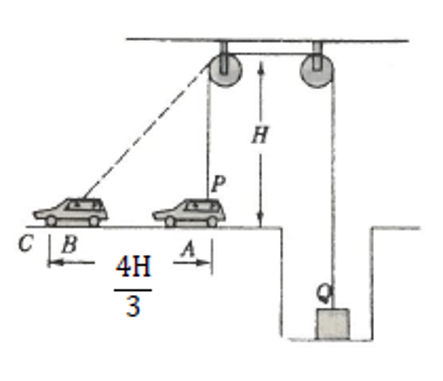
\includegraphics[width=0.25\textwidth]{109中女17.png}
\end{figure}
\newpage
%%%%%%%%%%%%%%%%%%%%%%%%%%%%%%%%%%%%%%%%%%%%%%%%%%%%%%%%%%%%%%%%%%%%%%%%%%%%%%%%%%%%

%%%%%%%%%%%%%%%%%%%%%%%%%%%%%%%%%%%%%%%%%%%%%%%%%%%%%%%%%%%%%%%%%%%%%%%%%%%%%%%%%%%%
\begin{example}
  如圖所示,一質量為M的直角三角形木塊,高度為h,斜角為$\theta$,起始時靜止於光滑的水平桌面上,
  另一質量為m的小木塊,放置於直角三角形木塊的頂端,自靜止開始下滑,假設兩木塊接觸面之間皆光滑,
  重力加速度為g,則滑動過程中,m相對於M的加速度為何?\\
  \rightline{[台中女中教甄109]} 
\end{example}
\begin{solution}
  $\frac{M+mg\sin\theta}{M+m\sin ^2 \theta}$
\end{solution}
\begin{figure}[htbp]
  \flushright
  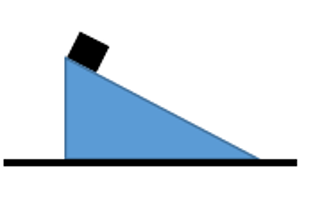
\includegraphics[width=0.25\textwidth]{109中女18.png}
\end{figure}
\newpage
%%%%%%%%%%%%%%%%%%%%%%%%%%%%%%%%%%%%%%%%%%%%%%%%%%%%%%%%%%%%%%%%%%%%%%%%%%%%%%%%%%%%


\section{計算題}



\begin{example}
如右圖所示,O 為某均質星球的球心,A、B 兩點為其北極與南極,$R$ 為半徑,$\rho$為
質量密度。今通過AOB 挖出一小條光滑通道,將質量為$m$ 的小球放入此通道,$m$ 遠小於
星球質量,在通道中的運動可視為一個質點。只考慮小球受到此星球的萬有引力,不必
考慮其餘阻力或星球的自轉與公轉效應,萬有引力常數以$G$ 表示,試回答以下各小題:
\begin{enumerate}[label=(\arabic*)] 
  \item 先後將兩個上述一樣的小球P、 Q 由A 點靜止自由釋放,兩球在C 點發生碰撞,$\overline{OC} = \frac{R}{2}$,則兩小球釋放的時間間隔為何?(3 分,答案請以$G、\rho、\pi $表示)
  \item 承上題,若兩小球碰撞的恢復係數為$e (0< e <1)$,碰撞後小球P 朝南極移動但在D 點即折返,試問D 與O 之間的距離。(3 分,答案請以$R$ 與$e$ 表示)
  \item 此後兩小球還會在通道中反覆碰撞,經過一段足夠長的時間之後,兩小球應處於什麼狀態? (4 分)
    \end{enumerate}
    \rightline{[台中女中教甄109]}
\end{example}
\begin{solution}
    
\end{solution}
\begin{figure}[htbp]
    \flushright
    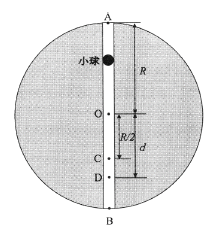
\includegraphics[width=0.3\textwidth]{image/109中女21.png}
  \end{figure}
\newpage




\begin{example}
   如圖所示,一質量為10 公斤,半徑為0.05 公尺的均質圓柱在一傾角為30$^\circ$的斜面
上被一條不可伸長的輕繩纏繞在圓柱上,並跨過無摩擦的滑輪在另一端連著一個質量為
20 公斤的重物。假設圓柱只滾不滑,求:(重力加速度為$g$)

\begin{enumerate}[label=(\arabic*)] 
  \item 試證明圓柱沿通過圓心軸(軸垂直其圓面)的轉動慣量為($M$ 為圓柱質量,$R$ 為圓
柱的圓半徑)(3 分)
  \item 圓柱中心的加速度。(3 分,答案請以$g$ 表示)
  \item 作用在接觸點P 上的靜摩擦力。(4 分,答案請以$g$ 表示)
    \end{enumerate}
    \rightline{[台中女中教甄109]}
\end{example}
\begin{solution}
    
\end{solution}
\begin{figure}[htbp]
    \flushright
    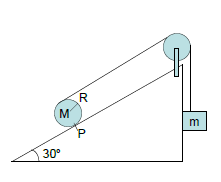
\includegraphics[width=0.3\textwidth]{image/109中女22.png}
  \end{figure}
\newpage


\begin{example}
   若有一個邊長20 公分,質量為960 公克的正立方體木塊恰靜止於半空中
時,有一顆質量40 公克子彈在木塊下方以200$m/s$ 鉛直向上以情境一或情境二
的方式射入木塊。情境一為子彈的速度延伸線通過木塊質心;情境二為子彈射向
木塊的邊緣中點。(已知子彈不會穿透木塊、空氣阻力可忽略、重力加速度為10
$m/s^2$、正立方體沿通過質心且垂直立方體之平面的軸旋轉時轉動慣量為$\frac{1}{6} ML^2$)
\begin{enumerate}[label=(\arabic*)] 
  \item 在情境一中,木塊可達到的最大高度為何?(3 分)
  \item 在情境二中,子彈射入木塊後,木塊旋轉的角速度約為何?(3分)(設子彈相較於木塊的體積很小,子彈射入木塊後對木塊造成的密度改變可以忽略)
  \item 某生作實驗發現,情境一與情境二其最大高度差異不大。但木塊邊上升邊轉動,除了移動動能外還有轉動動能,兩種情境能量皆由子彈轉換而來,而子彈所具有的初始動能皆相同,請說明為何實驗做出來兩種情境的最大高度相差不大,而情境二多出來的轉動動能又從何而來?(4 分)
    \end{enumerate}


    \rightline{[台中女中教甄109]}
\end{example}
\begin{solution}
    $(2)送分$
\end{solution}
\begin{figure}[htbp]
    \flushright
    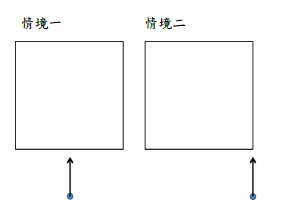
\includegraphics[width=0.3\textwidth]{image/109中女23.png}
  \end{figure}
\newpage



\begin{example}
   如右圖所示,要使一質量為$m$,帶$+q$的小球能水平沿直線加速,需要外加一均勻電場,已知
平行金屬板間距為$d$,與水平面夾角為$\theta$,要使此小球從A板左端沿直線從靜止沿水平方向被加
速,恰從B板射出,則(重力加速度為$g$)
\begin{enumerate}[label=(\arabic*)] 
  \item 兩金屬板間所加電壓$V$ 是多少?(5 分)
  \item 小球從B板射出時的速度是多大?(5 分)
    \end{enumerate}

    \rightline{[台中女中教甄109]}
\end{example}
\begin{solution}
    
\end{solution}
\begin{figure}[htbp]
    \flushright
    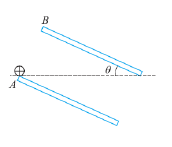
\includegraphics[width=0.3\textwidth]{image/109中女24.png}
  \end{figure}
\newpage






\chapter{成德高中}


\section{單選題}


\begin{example}
  1.在如圖所示的電路中,伏特計的內電阻為300歐姆、安培計的內電阻為5歐姆。
  電路中的電阻$R$ = 75歐姆、電阻$R_0$ = 115歐姆、理想電池的電動勢$\varepsilon $=12伏特,則伏特計的讀數為多少伏特?\\
  (A)2 (B)4 (C)6 (D)8 (E)9。\\
  \rightline{[成德高中教甄109]}
\end{example}
\begin{solution}
  
\end{solution}
\begin{figure}[htbp]
    \flushright
    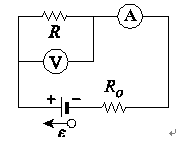
\includegraphics[width=0.3\textwidth]{image/109成德1.png}
  \end{figure}
\newpage



\begin{example}
  2.	空間中有水平方向的均勻電場,電場強度為E。在水平且光滑的絕緣平面上有一根長為$l$的無質量絕緣細桿,
  細桿兩端各有一個質量為$m$、帶等量異性電的小球A和B,電量均為$q$。開始時細桿方向平行於電場方向,如圖所示。
  讓這兩個帶電小球由靜止開始受靜電力作用(重力可忽略)而順時針繞細桿中心C點旋轉90$^\circ$瞬間,系統的總角動量大小為?\\
  (A) $\sqrt{\frac{1}{2} mqE l^3}$ (B) $\sqrt{mq E l^3}$ (C) $\sqrt{2mqE l^3}$ (D) $\sqrt{\frac{m l^3}{qE}}$ (E) $\sqrt{\frac{qE l^3}{2m}}$ \\
  \rightline{[成德高中教甄109]}
\end{example}
\begin{solution}
  
\end{solution}
\begin{figure}[htbp]
    \flushright
    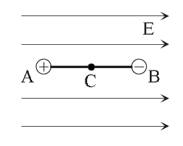
\includegraphics[width=0.2\textwidth]{image/109成德2.png}
\end{figure}

\newpage



\begin{example}
   3.將各50公克0$^\circ$C的冰及水,與各25公克100$^\circ$C的水及水蒸氣混合,假定此系統沒有任何熱量的損失,則經過一段時間後,此混合物的物態及溫度為何?
   (A)冰水共存,溫度0$^\circ$C(B)都化為水,溫度約為27$^\circ$C(C)都化為水,溫度約為77$^\circ$C(D)都化為水,溫度約為97$^\circ$C(E)水蒸氣及水共存,溫度100$^\circ$C
   \\
    \rightline{[成德高中教甄109]}
\end{example}
\begin{solution}
    
\end{solution}

\newpage


\begin{example}
   4.三稜鏡的主截面為正三角形,即每角均為60$^\circ$,稜鏡之折射率為n,今光線由一邊射入,另一邊射出,則最小入射角之正弦值為何?\\
   (A)$\sqrt{2 (n^2 - 1)}$ (B)$\sqrt{3 (n^2 - 1)}$ (C)$\frac{1}{2} (\sqrt{3 (n^2 - 1)}-1)$ (D)$\frac{1}{3} (\sqrt{2 (n^2 - 1)}-1)$ (E)$\frac{1}{2} (\sqrt{3 (n^2 - 1)})$
   \\
    \rightline{[成德高中教甄109]}
\end{example}
\begin{solution}
    
\end{solution}

\newpage

\begin{example}
   5.長度2$l_0$之密閉圓柱筒,中間以一極薄、可活動的隔板隔開,右邊裝1 $mol$之理想單原子分子氣體,筒之左側為真空,
   但置有一彈簧,彈簧之自然長度為2$l_0$,兩端分別固定在圓柱筒的左壁及隔板上,當絕對溫度為$T$時,隔板呈靜力平衡,
   且左右兩室體積等,如圖所示,則此彈簧的彈力常數為?\\
   (A)$\frac{RT}{l_0}$ (B)$\frac{RT}{l_0^2}$ (C)$\frac{l_0}{RT}$ (D)$\frac{l_0^2}{RT}$ (E)$RTl_0$\\
    \rightline{[成德高中教甄109]}
\end{example}
\begin{solution}
    
\end{solution}
\begin{figure}[htbp]
    \flushright
    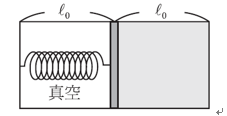
\includegraphics[width=0.3\textwidth]{image/109成德5.png}
  \end{figure}
\newpage


\begin{example}
   6.在一水平桌面上,一長度1.3$m$之細繩一端繫一物體,另一端則繫在長度亦為1.3$m$,以一端為軸旋轉的木棒上,
   如圖所示(由上方俯視)。若木棒轉動的角速度為2$rad/s$時,恰可使物體作半徑為2.4$m$的等速率運動,
   則物體與桌面間的動摩擦係數為?(g = $10m/s^2$)
   (A)0.2(B)0.4(C)0.5(D)0.6(E)0.8\\
    \rightline{[成德高中教甄109]}
\end{example}
\begin{solution}
    
\end{solution}
\begin{figure}[htbp]
    \flushright
    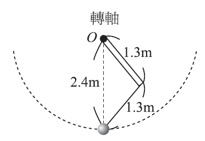
\includegraphics[width=0.3\textwidth]{image/109成德6.png}
  \end{figure}
\newpage

\begin{example}
   7.一水池內裝有折射率為$\frac{5}{3}$的液體,今將一點光源從液體表面由靜止開始釋放,此光源恰以等速度垂直向下運動。觀察者於液面發現,當光源逐漸往下沈時,射出液體表面的光所形成的圓面積就逐漸擴大。當光圓半徑為7.5公分瞬間開始計時,再經過3秒,光圓半徑變為30公分,則點光源下沈的速度為多少公分/秒?
   (A)2.5(B)5.0(C)7.5(D)10.0(E)12.5
   \\
    \rightline{[成德高中教甄109]}
\end{example}
\begin{solution}
    
\end{solution}

\newpage

\begin{example}
   8.一質量為m,帶電量為$q$的質點在一均勻磁場內作半徑為$R$的等速率圓周運動,如圖所示,當其運動到$K$點時,突然與一質量為2$m$的不帶電靜止粒子碰撞並合為一體,若碰撞後仍然作等速率圓周運動,其半徑為何?
   (A)$\frac{R}{3}$ (B)$\frac{2R}{3}$ (C)$R$ (D)$\frac{3R}{2}$ (E)$3R$
   \\
    \rightline{[成德高中教甄109]}
\end{example}
\begin{solution}
    
\end{solution}
\begin{figure}[htbp]
    \flushright
    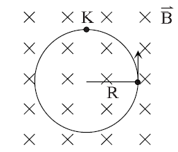
\includegraphics[width=0.3\textwidth]{image/109成德8.png}
  \end{figure}
\newpage

\begin{example}
   9.組成星球的物質是靠萬有引力吸引在一起。星球有最大的自轉速率,如果超過此速率,萬有引力將不足以維持赤道附近的物體做圓周運動。
   今若由上述得到半徑為$R$,密度為$\rho$,質量均勻分布,且質量為$M$的星球,萬有引力常數為$G$,其最大自轉速率為$v$。
   則$v$為下列何者?\\
   (A)$\sqrt{\frac{GM}{R^2}}$ (B)$\sqrt{\frac{4 \pi \rho G R^2}{3}}$ 
   (C)$\sqrt{\frac{4 \pi \rho  R}{3G}}$ (D)$\sqrt{\frac{GMR}{3 \rho}}$ (E)$\sqrt{\frac{3G}{\rho}}$
   \\
    \rightline{[成德高中教甄109]}
\end{example}
\begin{solution}
    
\end{solution}

\newpage

\begin{example}
   10.有一個邊長為$4a$的正方形均勻薄板,從薄板上切下一個半徑為$a$的圓形,如下圖所示。試問切割後的薄板質心位置距離$O$點多遠?
   (A)$\frac{\pi}{16-\pi}a$ (B)$\frac{\pi}{16}a$ (C)$\frac{\pi}{8-2\pi}a$ 
   (D)$\frac{\sqrt{2} \pi}{16-\pi}a$ (E)$\frac{\sqrt{2} \pi}{16-4\pi}a$\\
    \rightline{[成德高中教甄109]}
\end{example}
\begin{solution}
    
\end{solution}
\begin{figure}[htbp]
    \flushright
    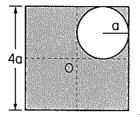
\includegraphics[width=0.3\textwidth]{image/109成德10.png}
  \end{figure}
\newpage

\begin{example}
   11.如圖所示,在高度10$m$的高塔上,以仰角30$^\circ$及$v_A$的初速率拋出A球,而同一時間,在A球正下方塔底位置有一B球,
   以仰角60$^\circ$及$v_B$的初速率拋出,A與B的運動軌跡在同一平面上。不計空氣阻力,若想讓A、B兩求在空中相遇,
   請問$v_A$需符合下列哪一個條件?\\
   (A)$v_A > \frac{10\sqrt{3}}{3}$ (B)$v_A < \frac{10\sqrt{3}}{3}$ (C)$v_A > 10\sqrt{3}$ 
   (D)$v_A < 10\sqrt{3}$ (E)$v_A > 5\sqrt{3}$\\
    \rightline{[成德高中教甄109]}
\end{example}
\begin{solution}
    
\end{solution}
\begin{figure}[htbp]
    \flushright
    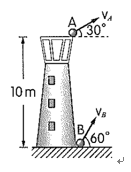
\includegraphics[width=0.3\textwidth]{image/109成德11.png}
  \end{figure}
\newpage


\begin{example}
   12.如圖所示,質量分別為$m_1$和$m_2$的兩個小木塊分別套在光滑的水平桿上,以長度為$l$的細線連接,水平桿隨框架以角速度$\Omega$做等角速度轉動,而兩木塊相對於水平桿恰為靜止。求細線的拉力為:
   (A)$\frac{m_1 m_2}{m_1 +m_2} \omega^2 l$ (B)$\frac{2 m_1 m_2}{m_1 +m_2} \omega^2 l$
   (C)$\frac{m_1 m_2}{2(m_1 +m_2)} \omega^2 l$ (D) $\frac{m_1(m_1 +m_2)}{m_2} \omega^2 l$
   (E)$\frac{m_2(m_1 +m_2)}{m_1} \omega^2 l$
   \\
    \rightline{[成德高中教甄109]}
\end{example}
\begin{solution}
    
\end{solution}
\begin{figure}[htbp]
    \flushright
    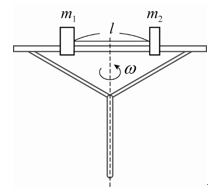
\includegraphics[width=0.3\textwidth]{image/109成德12.png}
  \end{figure}
\newpage

\begin{example}
   13.有一太空船飛至地球與月球之間某處時,發現引力恰為零。此時太空人望向地球,發現視角為$\theta$;望向月球,發現視角為2$\theta$;則地球與月球的質量比為何?(設地球與月球密度相同,且地球與月球距離遠大於兩者之半徑)
   (A)8:1 (B)16:1 (C)32:1 (D)64:1 (E)128:1。
   \\
    \rightline{[成德高中教甄109]}
\end{example}
\begin{solution}
    
\end{solution}

\newpage

\begin{example}
   14.如圖所示,在平面直角坐標系中有一個垂直紙面向內的圓形均勻磁場,其邊界過原點$O$和$y$軸上的點$a(0_,L)$ ,一質量為$m$、電荷量為$e$的電子從a點以初速度$V_0$平行於$x$軸正方向射入磁場,並從$x$軸上的$b$點射出磁場,此時速度方向與$x$軸正方向的夾角為60$^\circ$。假設磁場區域的圓心為$O_1$,電子在磁場所作的圓周運動的圓心為$O_2$,則$O_1$與$O_2$間的距離為
   (A)0 (B)$\frac{L}{2}$ (C)$\frac{L}{\sqrt{3}}$ (D)$\sqrt{2} L$ (E)$\sqrt{3} L$
   \\
    \rightline{[成德高中教甄109]}
\end{example}
\begin{solution}
    
\end{solution}
\begin{figure}[htbp]
    \flushright
    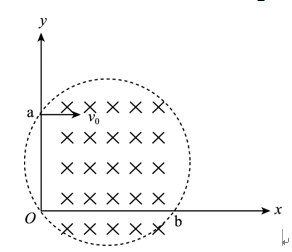
\includegraphics[width=0.3\textwidth]{image/109成德14.png}
  \end{figure}
\newpage


\begin{example}
   15.如圖(a),水平置放的粗細均勻的玻璃管內含有$L_0$公分的水銀柱,在大氣壓力為$h_0$公分-水銀汞柱時,
   封閉兩端使左右兩氣室體積相等。若玻璃管作水平等加速度直線運動,使右室氣體體積為左室的$y$倍($y>1$),
   如圖(b),則玻璃管的加速度為何?($g$為重力加速度)\\
   (A)$\frac{(y^2 -1)}{2y} \frac{h_0}{L_0} g$( B)$\frac{(y -1)}{2y} \frac{h_0}{L_0} g$ 
   (C)$\frac{(y^2 -1)}{y} \frac{h_0}{L_0} g$ (D)$\frac{2(y -1)}{y} \frac{h_0}{L_0} g$ 
   (E)$\frac{2(y -1)}{y^2} \frac{h_0}{L_0} g$
   \\
    \rightline{[成德高中教甄109]}
\end{example}
\begin{solution}
    
\end{solution}
\begin{figure}[htbp]
    \flushright
    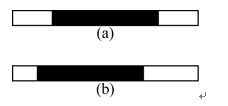
\includegraphics[width=0.3\textwidth]{image/109成德15.png}
  \end{figure}
\newpage



\begin{example}
  16.一個內部填充氦氣的氣球,由地面升到高空。假設高空的氣壓為地面處的一半,
  但高空與地面處的溫度相同,若氣球表皮的張力可不計,則在每單位時間內碰撞到氣球表面積上的氦分子數為地面處的
(A)2$^{\frac{-1}{3}}$ (B)2$^{-1}$ (C)2 (D)2$^\frac{-2}{3}$ (E)2$^\frac{-4}{3}$ 倍
  \\
    \rightline{[成德高中教甄109]}
\end{example}
\begin{solution}
    
\end{solution}

\newpage

\begin{example}
   17.有一氣體噴嘴以速率$v$噴出分子質量為$m$的氣體,其單位體積內含有分子數為$n$,
   若氣體分子以入射角$\theta$撞擊一牆壁,撞擊視為彈性碰撞,則牆壁所受氣體之壓力為若干?\\
   (A)$2nmv^2 \cos^2{\theta}$ (B)$2nmv^2 \cos{\theta}$ (C)$nmv^2 \cos^2{\theta}$ 
   (D)$nmv^2 \cos{\theta}$ (E)$2nmv \cos{\theta}$
   \\
    \rightline{[成德高中教甄109]}
\end{example}
\begin{solution}
    
\end{solution}

\newpage

\begin{example}
   18.附圖為一光纖之側面剖面圖,其中$n_1$及$n_2$分別代表不同物質之折射率,
   $n_1$之部分稱為核心。若要使光在核心中靠全反射傳遞(不穿透$n_1$介質而產生漏失),
   $\sin{\theta}$須小於下列哪一個值?\\
   (A)$n_1 \sqrt{1-\frac{n_2}{n_1}}$ (B)$n_2 \sqrt{1-(\frac{n_2}{n_1}^2}$ 
   (C)$n_1 \sqrt{1-\frac{n_2}{n_1}}$ (D)$n_2 \sqrt{1-(\frac{n_2}{n_1})^2}$ 
   (E)$\sqrt{n_1 n_2(1-\frac{n_2}{n_1})}$
   \\
    \rightline{[成德高中教甄109]}
\end{example}
\begin{solution}
    
\end{solution}
\begin{figure}[htbp]
    \flushright
    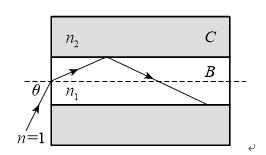
\includegraphics[width=0.3\textwidth]{image/109成德18.png}
  \end{figure}
\newpage

\begin{example}
   19.如附圖,焦距為20公分之凸透鏡自主軸分成兩半後再相距2.0$\times10^{-2}$公分,其間以不透光之物體遮住。在透鏡前30公分處置一波長為600奈米的點光源$S$,則距透鏡210公分處之光屏上所形成的干涉條紋中,第二亮紋與中央軸線最近距離為
   (A)0.10 (B)0.15 (C)0.20 (D)0.25 (E)0.30 公分。
   \\
    \rightline{[成德高中教甄109]}
\end{example}
\begin{solution}
    
\end{solution}
\begin{figure}[htbp]
    \flushright
    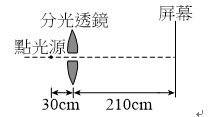
\includegraphics[width=0.3\textwidth]{image/109成德19.png}
  \end{figure}
\newpage

\begin{example}
   20.質量為2公斤、半徑為$R$的均勻圓環靜置於光滑水平桌面上,另有一質量為3公斤的物體置於圓心處。若物體爆炸成質量比為2:1的兩片,且分別向左、向右黏住於環上,則最後環之位移大小為若干?
   (A)$\frac{1}{5}R$(B)$\frac{2}{5}R$(C)$\frac{R}{2}$(D)$\frac{3}{5}R$(E)$\frac{4}{5}R$
   \\
    \rightline{[成德高中教甄109]}
\end{example}
\begin{solution}
    
\end{solution}

\newpage


\begin{example}
   21.在低空水平拋出一物,經$t$秒後其運動之法向加速度與切向加速度之大小相等。不計空氣阻力,再經幾秒法向加速度為切向加速度的一半?
   (A)$\frac{t}{2}$ (B)$\frac{\sqrt{2}}{2}t$ (C)$t$ (D)$\sqrt{2}t$ (E)$2t$
   \\
    \rightline{[成德高中教甄109]}
\end{example}
\begin{solution}
    
\end{solution}

\newpage


\begin{example}
   22.一砲彈在地面上以初速100公尺/秒,仰角37$^\circ$發射,當砲達最高點時即爆裂為質量相等之A、B兩塊,
   其中一塊A於砲彈爆裂後8秒著地,則另一塊B著地較塊A(g = 10公尺/$秒^2$)\\
   (A)早6.5秒 (B)早5.0秒 (C)早3.5秒 (D)晚3.5秒 (E)晚0.5秒。
   \\
    \rightline{[成德高中教甄109]}
\end{example}
\begin{solution}
    
\end{solution}

\newpage


\begin{example}
  23.一汽車(含駕駛、乘客)質量2000公斤,引擎輸出功率為22千瓦,恰可在仰角$\sin^{-1}{\frac{1}{10}}$ 的斜坡上,
  以10公尺/秒等速爬坡。若重力加速度10公尺/$秒^2$,則摩擦阻力之量值為\\
  (A)200 (B)100 (C)80 (D)50 (E)20 牛頓。
\\
    \rightline{[成德高中教甄109]}
\end{example}
\begin{solution}
    
\end{solution}

\newpage


\begin{example}
   24. A、B兩物的質量比$m_A:m_B=$1:2,用理想輕彈簧連結在一起,放在光滑水平地面上,A物體靠在牆邊,如圖所示。用力向左推B物體,壓縮彈簧,外力對其作功為120焦耳時,突然撤去外力,從A物體開始向右運動以後,彈簧彈性位能的最大值為多少焦耳? (A)40 (B)60 (C)80 (D)90 (E)120。\\
    \rightline{[成德高中教甄109]}
\end{example}
\begin{solution}
    
\end{solution}
\begin{figure}[htbp]
    \flushright
    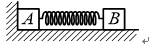
\includegraphics[width=0.3\textwidth]{image/109成德24.png}
  \end{figure}
\newpage



\begin{example}
   25.有一均勻帶電圓環,帶電量為$+Q(Q>0)$,半徑為$R$,質量為$M$,圓周率為$\pi$。
   今將此圓環放在絕緣光滑水平桌面上,並有均勻磁場$B$作用,其方向為垂直向下射入桌面。
   當此圓環通過其中心的鉛直軸以等轉速$\omega$旋轉時(觀察者由上往下俯視,圓環為逆時針旋轉),請問圓環中的張力為?\\
   (A)$\frac{2\pi}{R\omega}(M\omega-QB)$ (B)$\frac{2\pi}{R\omega}(M\omega+QB)$ 
   (C)$\frac{R\omega}{2\pi}(M\omega-QB)$ (D)$\frac{QR\omega B}{2\pi}$ (E)$\frac{MR^2\omega}{2\pi}$
   \\
    \rightline{[成德高中教甄109]}
\end{example}
\begin{solution}
    
\end{solution}

\newpage


\begin{example}
   26. 如圖所示,質量為$m$,帶有正電荷的小球繫於長為$L$的細繩的一端,細繩的另端固定在O點。
   假設空間中有水平向右的均勻電場,重力場大小為$g$方向向下,小球在圖示位置P點呈靜平衡狀態,
   此時細繩與鉛垂線夾53$^\circ$角。若要使小球自P點出發能繞O點旋轉一周,則小球在P點的初速最小為\\
(A)$\sqrt{\frac{7}{4}gL}$ (B)$\sqrt{\frac{14}{4}gL}$ (C)$\sqrt{\frac{14}{3}gL}$ 
(D)$\sqrt{\frac{25}{4}gL}$ (E)$\sqrt{\frac{25}{3}gL}$
\\
    \rightline{[成德高中教甄109]}
\end{example}
\begin{solution}
    
\end{solution}
\begin{figure}[htbp]
    \flushright
    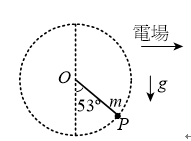
\includegraphics[width=0.3\textwidth]{image/109成德26.png}
  \end{figure}
\newpage


\begin{example}
   27. 有二電阻器$R_1$、$R_2$可以並聯或串聯組合,跨過電動勢$\varepsilon$之電池,
   內電阻不計,欲使並聯組合之電功率為串聯組合之4.5倍,若$R_1 =$ 100歐姆,則$R_2$為若干歐姆?($R_1 > R_2$)  \\
   (A)90 (B)80 (C)75 (D)60 (E)50  歐姆。\\
    \rightline{[成德高中教甄109]}
\end{example}
\begin{solution}
    
\end{solution}

\newpage


\begin{example}
   28. 有一以$O$為圓心、$L$為半徑的$OMN$扇形電路置於均勻磁場$B$中如圖所示,
   磁場垂直穿入紙面,半徑$OM$之間有電阻$R$,電路中其他電阻可忽略不計。$OM$與$MP$弧固定不動,
   而長度為$L$的$ON$以$O$為軸心作順時針往$P$方向旋轉,角速率為$\omega$,則電路中電流為下列何者?\\
   (A)$\frac{\omega BL^2}{2R}$ (B)$\frac{\omega B^2 L^2}{2R}$ 
   (C)$\frac{\omega BL}{R}$ (D)$\frac{\omega BL^2}{R}$ (E)$\frac{\omega^2 BL^2}{R}$
   \\
    \rightline{[成德高中教甄109]}
\end{example}
\begin{solution}
    
\end{solution}
\begin{figure}[htbp]
    \flushright
    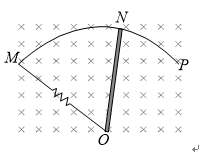
\includegraphics[width=0.3\textwidth]{image/109成德28.png}
  \end{figure}
\newpage


\begin{example}
   29.欲將原為電中性的氦原子中兩個電子完全除去所需的總能量為79電子伏特,則當氦原子僅除去第一個電子時需要能量為若干?(A)65.4 (B)51.8 (C)38.2 (D)24.6 (E)13.6 電子伏特。\\
    \rightline{[成德高中教甄109]}
\end{example}
\begin{solution}
    
\end{solution}

\newpage


\begin{example}
  30.在特殊實驗環境下,假設直線運動的鈉原子(原子量23)速率為$300m/s$,今以波長為5890埃的雷射光正面照射它,
  知質子的質量為$m_p=1.67 \times 10^{-27} kg$、普郎克常數為$h= 6.63 \times 10^{-34} Js$,
  試算此鈉原子約要吸收多少個光子就會停下來?(朱棣文博士之光冷卻原子理論)\\
  (A)10 (B)$10^4$ (C)$10^6$ (D)$10^9$ (E)$10^12$。 \\
    \rightline{[成德高中教甄109]}
\end{example}
\begin{solution}
    
\end{solution}

\newpage


\begin{example}
   31.如圖所示,A點為聲源發出聲波,波長為1公尺,在其下方距10公尺的地方有一反射面可反射聲波,則聲源右方20公尺有一觀察者阿凱在B點,若阿凱直直往下走向反射面,則阿凱可聽到幾個無聲音的地方?(反射面上的不算)(A)16 (B)14 (C)12 (D)8 (E)6 個。\\
    \rightline{[成德高中教甄109]}
\end{example}
\begin{solution}
    
\end{solution}
\begin{figure}[htbp]
    \flushright
    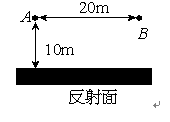
\includegraphics[width=0.3\textwidth]{image/109成德31.png}
  \end{figure}
\newpage



\begin{example}
   32.一管子兩端開口時,可產生頻率為800赫茲的聲波,如將一端封閉時,可產生頻率為200赫茲的聲波,設聲速為320公尺/秒,則管長的最小值為 (A)1.6 (B)1.0 (C)0.8 (D)0.4 (E)0.2  公尺。\\
    \rightline{[成德高中教甄109]}
\end{example}
\begin{solution}
    
\end{solution}

\newpage


\begin{example}
   33.學生翔智做實驗,在教學大樓走廊側離地$h=60m$處,將一小球靜止自由釋放下落,小球著地後又彈起、又落下。經測量後,小球每次與地面相碰後,彈起速率為著地速率的$\frac{1}{2}$,不計空氣阻力, $g=10 m/s^2$,試問小球全程運動的總路徑長為多少m?(A)150 (B)120 (C)105 (D)100 (E)90。\\
    \rightline{[成德高中教甄109]}
\end{example}
\begin{solution}
    
\end{solution}

\newpage

\begin{example}
   34.隔離系統中,有一邊長為$a$的正方形的載電流$I$導線框,請問此正方形之中心O處的磁場強度為若干? 
   (A)$\frac{4\mu_0 I}{\pi a}$ (B)$\frac{2\sqrt{2} \mu_0 I}{\pi a}$ (C)$\frac{2\mu_0 I}{\pi a}$ (D)$\frac{\sqrt{2}\mu_0 I}{\pi a}$
    (E)$\frac{\sqrt{2}\mu_0 I}{2pi a}$
   \\
    \rightline{[成德高中教甄109]}
\end{example}
\begin{solution}
    
\end{solution}
\begin{figure}[htbp]
    \flushright
    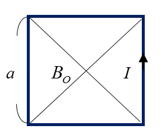
\includegraphics[width=0.3\textwidth]{image/109成德34.png}
  \end{figure}
\newpage


\begin{example}
   35.在孤立系統中,有兩星體質量比為$1:4$,原相距$d$時萬有引力為$F$。兩星體原相距$d$從靜止狀態,藉由萬有引力牽引至相距$\frac{2}{3}d$時,請問質量較小者動能為若干?
   (A)$2Fd$ (B)$\frac{8}{5}Fd$ (C)$\frac{4}{5}Fd$ (D)$\frac{3}{5}Fd$ (E)$\frac{2}{5}Fd$
   \\
    \rightline{[成德高中教甄109]}
\end{example}
\begin{solution}
    
\end{solution}

\newpage

\section{多選題}

\begin{example}
   36.一台迴旋加速器用來加速質子(帶電量為$q$,質量為$m$),如圖所示,若兩半圓形(半徑為$R$)中通有均勻磁場$B$,
  中間是一極薄的平行電場,加速電壓$\Delta V$=$2.0\times10^4V$,質子每經過一次平行電場,
   便會被加速一次。若要將質子從加速器圓心,從靜止加速至磁場邊緣時共增加動能$K$=$4MeV$,則下列敘述何者正確?
   \begin{enumerate}[label=(\Alph*)]
     \item 圖中所示質子之二運動軌跡(半圓形),以半徑較大者,所花之時間較長
     \item 承(A),質子在此二運動軌跡之角速度大小相同
     \item 均勻磁場B之大小至少為$\frac{\sqrt{2mK}}{qR}$
     \item 質子要達到動能為$4MeV$,需電場加速至少200次以上
     \item 承(D),若質子在磁場中運行一完整圓之週期為$Ts$,則此次加速共需花200$Ts$ 
   \end{enumerate}
   
    \rightline{[成德高中教甄109]}
\end{example}
\begin{solution}
    
\end{solution}
\begin{figure}[htbp]
    \flushright
    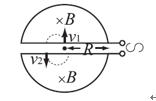
\includegraphics[width=0.3\textwidth]{image/109成德36.png}
  \end{figure}
\newpage



\begin{example}
   37.有五個完全相同燈泡a、b、c、d、e,連接於電路上,如圖所示,則:
   \begin{enumerate}[label=(\Alph*)]
    \item 流經b燈泡與c燈泡的電流比為$3:1$
    \item b燈泡與d燈泡兩端的電壓比為$3:1$
    \item a燈泡與b燈泡的功率比$25:9$
    \item 若將a燈泡拆除,則通過b燈泡的電流將會增加
    \item 若將c燈泡拆除,則通過b燈泡的電流將會增加
   \end{enumerate}

    \rightline{[成德高中教甄109]}
\end{example}
\begin{solution}
    
\end{solution}
\begin{figure}[htbp]
    \flushright
    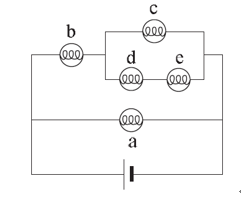
\includegraphics[width=0.3\textwidth]{image/109成德37.png}
  \end{figure}
\newpage


\begin{example}
   38.一定質量的理想氣體狀態變化的$V-T$圖如圖示,由狀態A經過B、C、D各狀態又回到狀態A,則:
   \begin{enumerate}[label=(\Alph*)]
     \item 狀態A到B,氣體對外作功,內能增加,密度減少
     \item 狀態B到C,氣體分子平均動能增加,密度減少
     \item 狀態C到D,氣體放熱,密度減少,分子平均動能不變
     \item 狀態D到A,氣體內能減少,氣體放熱
     \item 狀態B到C與狀態D到A氣體壓力均保持不變,但B到C過程壓力小於D到A過程的壓力
   \end{enumerate}

    \rightline{[成德高中教甄109]}
\end{example}
\begin{solution}
    
\end{solution}
\begin{figure}[htbp]
    \flushright
    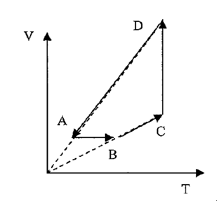
\includegraphics[width=0.3\textwidth]{image/109成德38.png}
  \end{figure}
\newpage


\begin{example}
   39.有A、B、C、D四種光照射同一光電板,其光電流與電壓之關係如圖,則 
   \begin{enumerate}[label=(\Alph*)]
     \item 光強度最大的為A
     \item 照射光子能量最大的為B
     \item 光束A射出之光電子動量最大
     \item 光速$A>B=C>D$
     \item 光子數量$B>A>C=D$
   \end{enumerate}

    \rightline{[成德高中教甄109]}
\end{example}
\begin{solution}
    
\end{solution}
\begin{figure}[htbp]
    \flushright
    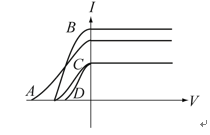
\includegraphics[width=0.3\textwidth]{image/109成德39.png}
  \end{figure}
\newpage



\begin{example}
   	40.一複合體由A、B兩大小相同的正立方體木塊(邊長為$d$)所構成,如下左圖所示。若A的密度為$\rho$,
     B的密度為$\frac{2}{3}\rho$,O為複合體的幾何中心,P、Q皆位於邊長中點,則下列哪些敘述是正確的?
     \begin{enumerate}[label=(\Alph*)]
       \item A、B兩木塊的質量比為$3:2$
       \item 複合體的共同質心距離O點$\frac{2}{5}d$
       \item 若以P為懸吊點,將複合體吊起,下右圖所示,達平衡後$\tan{\theta} = \frac{5}{9}$
       \item 若改以Q為懸吊點,$\theta$不會改
       \item 以P為懸吊點的情形下,將B木塊鋸掉,新的平衡狀態下$\tan{\theta} = \frac{1}{2}$
     \end{enumerate}

    \rightline{[成德高中教甄109]}
\end{example}
\begin{solution}
    
\end{solution}
\begin{figure}[htbp]
    \flushright
    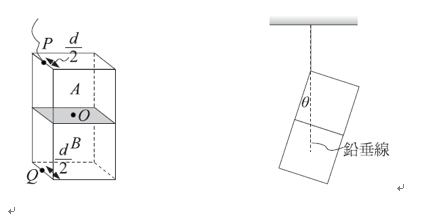
\includegraphics[width=0.4\textwidth]{image/109成德40.png}
  \end{figure}
\newpage



\section{計算題}

\begin{example}
   1.	巴拿馬運河的寬度為$W$,因此水閘門寬度也是$W$,水閘門兩邊運河水的深度分別為$h_1$和$h_2 (ℎ_1 > ℎ_2)$,如圖所示,則:
   \begin{enumerate}[label=(\arabic*)] 
\item 兩側的水作用在水閘門的靜力和為何?  $( 3\% )$
\item 如以通過水閘門的底部和水閘門平行的線作為轉軸,則作用在水閘門的力矩大小為何?  $( 2\% )$
(設水閘門的厚度可以忽略不計,水的密度為$\rho$,重力加速度為$g$。)
\end{enumerate}

    \rightline{[成德高中教甄109]}
\end{example}
\begin{solution}
    
\end{solution}
\begin{figure}[htbp]
    \flushright
    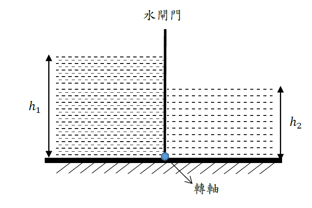
\includegraphics[width=0.3\textwidth]{image/109成德41.png}
  \end{figure}
\newpage



\begin{example}
   	2.現討論彈簧縱波(壓縮波)的波速與彈簧特性(彈性係數$k$,全長$L$,截面積為$A$,總質量$M$)的關係。已知在介質中壓縮波(縱波)的速度為$v=\sqrt{\frac{B}{\rho}})$,其中$\rho$為介質密度,$B$為體積係數。$B$為施加壓力與體積變化之間的係數,其定義為關係$ \Delta P\equiv-B \frac{\Delta V}{V}$其中$V$為被壓縮物體的體積,$\Delta P$為作用在物體的壓力,$\Delta V$為相對應壓力$\Delta P$所產生的體積變化。將此彈簧兩端固定,並在彈簧的一端施加固定頻率之外力(如音叉),討論其波動現象。
   	\begin{enumerate}[label=(\arabic*)] 
\item 體積係數$B$與彈簧的彈性係數$k$、全長$L$的關係為何?$( 3\% )$
\item 壓縮波(縱波)的波速與波長的關係為何?  $( 2\%)$
\end{enumerate}
    \rightline{[成德高中教甄109]}
\end{example}
\begin{solution}
    
\end{solution}

\newpage



\begin{example}
   3.在波耳的氫原子結構理論中,請推導出下列各物理量與量子數$n$的關係?
   \begin{enumerate}[label=(\arabic*)]
     \item 電子速率$( 2\%)$
     \item 電子軌道半徑$( 2\%)$
     \item 電子軌道運動的週期$( 1\%)$
      \end{enumerate}

    \rightline{[成德高中教甄109]}
\end{example}
\begin{solution}
    
\end{solution}

\newpage


\begin{example}
    簡諧運動週期。
    \begin{enumerate}[label=(\arabic*)]
        \item 有一U型管(內截面積大小恆定)內裝有均質液體,今以活塞在一邊暫時壓下液體一小段$x(x\ll L)$,
        瞬間移去活塞後,觀察到液面開始上下振盪,知$L$為管中液體全長,$g$為重力加速度,$\pi$為圓周率,
        請問振盪週期$T$為?$( 3\% )$
        \item 一均勻長方體木頭(長、寬、高分別為$a, b, h$)浮於水面時,有一半體積沉在水面下。若輕壓此木頭後放手,則此木頭在水面上會上下振盪。假設水與此木頭間無摩擦力,請問振盪週期$T$為?$( 2\%)$
    \end{enumerate}
    
    \rightline{[成德高中教甄109]}
\end{example}
\begin{solution}

\end{solution}
\begin{figure}[htbp]
    \flushright
    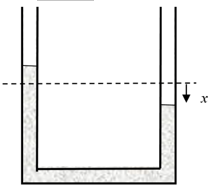
\includegraphics[width=0.3\textwidth]{image/109成德44.png}
  \end{figure}
\newpage



\chapter{文華高中109}
\section{填充題}

\begin{example}
   1.如右圖,在一傾斜角為$\alpha$的斜面上,以初速度$v_0$、與水平方向成$\beta$角斜向拋射一物體。假設斜面夠長,空氣阻力可忽略 ,重力加速度為$g$,則當$\beta$角為$\underline{  (1)  }$時 落點與原拋射點的距離$R$會有最大值。\\
    \rightline{[文華高中教甄109]}
\end{example}
\begin{solution}
    $\frac{\pi} {4}-\frac{\alpha} {2}$
\end{solution}
\begin{figure}[htbp]
    \flushright
    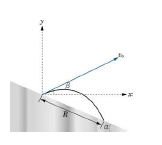
\includegraphics[width=0.3\textwidth]{image/109文華1.png}
  \end{figure}
\newpage


\begin{example}
   2.如右圖,一車以等加速度向右運動。假設木塊$m=3$公斤且與車間無摩擦,而木塊$ M =10 公斤$且 與車間的靜摩擦係數為$\mu=0.1$。若重力加速度$g=10m/s^2$則欲使車向右運動過程中$M$ 的高度保持不變,則車的加速度範圍應為$\underline{(2)}$。
   \\
    \rightline{[文華高中教甄109]}
\end{example}
\begin{solution}
    $25\le a \le 50  m/s^2 $
\end{solution}
\begin{figure}[htbp]
    \flushright
    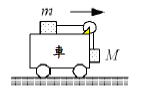
\includegraphics[width=0.3\textwidth]{image/109文華2.png}
  \end{figure}
\newpage


\begin{example}
   3.一個高度$h$的圓柱形水桶置於水平地面上,水桶內的水為滿水位則在水桶側面距地高度為$\underline{(3)}$處鑽一小孔,水由孔水平噴出所能達到的水平射程為最大(假設水與桶間的
表面張力可忽略) 。\\
    \rightline{[文華高中教甄109]}
\end{example}
\begin{solution}
    $\frac{h} {2}$
\end{solution}

\newpage


\begin{example}
   4.一個質量為$m$ 的帶電質點,在間距為$ L$的兩個固定壁間作一維運動,若普朗克常數為$h$,則此帶電 質點由第一受激態躍遷回基態的電磁輻射頻率為$\underline{(4)}$ 。\\
    \rightline{[文華高中教甄109]}
\end{example}
\begin{solution}
    $\frac{3h} {8mL^2}$
\end{solution}

\newpage


\begin{example}
   5.重量100$ kg$ 的台車靜止於光滑水平面上,其上載有2個質量均為50$kg$ 的人。若每人「相
繼」以同方向相對台車$ v$ 的水平速度跳離車,最後車速變為$v _1$ ,而若兩人「同時」以同方
向相對台車 $v$ 的水平速度跳離車,車速變為$v_2$ ,則 $\frac{v_2}{v_1}$ 之比值為$\underline{(5)}$ 。\\
    \rightline{[文華高中教甄109]}
\end{example}
\begin{solution}
    $\frac{6}{7}$
\end{solution}

\newpage

\begin{example}
   6.20個電阻如右圖連接,每個電阻值皆為$ R$ ,則 a 、 b 兩點間的等效
電阻值為$\underline{(6)} $ 。
\\
    \rightline{[文華高中教甄109]}
\end{example}
\begin{solution}
    $2R$
\end{solution}
\begin{figure}[htbp]
    \flushright
    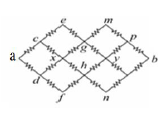
\includegraphics[width=0.4\textwidth]{image/109文華6.png}
  \end{figure}
\newpage


\begin{example}
   7.A質點自高度為$h$的樓頂頂端靜止落下,同時在同一鉛直線上的地面,有另一質點B自地
面向上以初速$v_0$鉛直上拋。已知兩質點在空中相遇時B質點正在向下運動,假設空氣阻力
可忽略、重力加速度為$ g$,則初速度$v_0$ 的範圍應為$\underline{(7)}$ 。
\\
    \rightline{[文華高中教甄109]}
\end{example}
\begin{solution}
    $\sqrt{\frac{1}{2} gh} < v_0 < \sqrt{gh}$
\end{solution}

\newpage


\begin{example}
   8.如右圖,一個質量為$ M$ 、斜角為$\theta$的斜面靜置於磅秤上,而質量為$m$ 的小木塊正在沿斜面下滑,木塊與斜面間無摩擦。假設木塊下滑過程中 斜
面保持靜止,重力加速度為$ g$,則此時磅秤的讀數為$\underline{(8)}$ 。
\\
    \rightline{[文華高中教甄109]}
\end{example}
\begin{solution}
    $(M+m)g-mg\sin^2 {\theta}$
\end{solution}
\begin{figure}[htbp]
    \flushright
    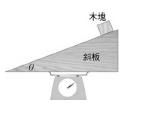
\includegraphics[width=0.3\textwidth]{image/109文華8.png}
  \end{figure}
\newpage


\begin{example}
   9.如右圖, 三根質量為$m$、長度皆為$L$的相同 均勻細 棒靠在一起, 且 三棒與
地面的接觸點 A 、 B 、 C 間 距皆為$L$ 假 設三棒與地面間的 靜 摩擦係數相
同 則 若要使系統保持靜力平衡, 棒與地面 間 的靜摩擦係數$\mu_s$ 最 小
值 為$\underline{(9)}$ 。
\\
    \rightline{[文華高中教甄109]}
\end{example}
\begin{solution}
    $\frac{\sqrt{2}} {4}$
\end{solution}
\begin{figure}[htbp]
    \flushright
    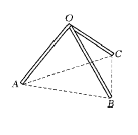
\includegraphics[width=0.3\textwidth]{image/109文華9.png}
  \end{figure}
\newpage


\begin{example}
   10.一木棒 A端靠在鉛直牆壁上,另一端 B 端 於 水平地面 上,則當棒由靜止下
滑至棒與水平成$\theta$角之瞬間, A 、 B 兩端的速率比值$\frac{v_A}{v_B}$ 為$\underline{(10)}$ 。 (假設下滑過程中 A 端保持與牆壁接觸 、 B 端保持與地面接觸)
\\
    \rightline{[文華高中教甄109]}
\end{example}
\begin{solution}
    $\cot{\theta}$
\end{solution}
\begin{figure}[htbp]
    \flushright
    \includegraphics[width=0.3\textwidth]{image/109文華10.png}
  \end{figure}
\newpage


\begin{example}
  11.
如右圖, 光滑水平面上置一質量為$m$,邊長為$9cm$的正方體木塊
一長為$25cm$的輕質光滑細桿,可繞下端固定在地面上的$O$點 自由 旋
轉,上端固定一質量亦為$m$的質點,桿子靠在木塊上,桿與木塊 間
無摩擦。 現將 桿子自與水平面夾角$\theta=53^\circ$靜止釋放,則當桿與水
平面夾角$\theta=37^\circ$ ,木塊的速率為$\underline{(11)}$公尺/秒(已知 重力
加速度 $g=10m/s^2$) \\
    \rightline{[文華高中教甄109]}
\end{example}
\begin{solution}
    $\frac{\sqrt{2}} {2}$
\end{solution}
\begin{figure}[htbp]
    \flushright
    \includegraphics[width=0.3\textwidth]{image/109文華11.png}
  \end{figure}
\newpage


\begin{example}
   12.如右圖,一質量為$ M$ 的光滑斜面靜止在光滑水平面上,今
有一質量為 $m$ 的小球以水平初速度$V$ 滑上斜面,假設小球
不會衝過斜面頂,則小球沿斜面上升到最大高度的過程中,
斜面對小球所做的功為$\underline{(12)}$。\\
    \rightline{[文華高中教甄109]}
\end{example}
\begin{solution}
    $- \frac{Mm^2}{2(M+m)^2} V^2$
\end{solution}
\begin{figure}[htbp]
    \flushright
    \includegraphics[width=0.3\textwidth]{image/109文華12.png}
  \end{figure}
\newpage


\begin{example}
  13.如右圖,將長度為$L$ 的均勻繩子置於水平桌面上,繩子與桌面 間 的 動、
靜 摩擦係數 皆 為 $\mu$將此繩拉直並慢慢拉出桌子,使一部分繩子靜止懸吊
在桌子邊緣 。 現 將懸吊在桌邊繩子的末端施一向下極微小的力,繩子隨即
向下滑落 ,則 整條繩子恰離開桌面時的速率為$\underline{(13)}$ 。 (重力加速度
為 $g$ ) \\
    \rightline{[文華高中教甄109]}
\end{example}
\begin{solution}
    $\sqrt{\frac{gL} {1+\mu}}$
\end{solution}
\begin{figure}[htbp]
    \flushright
    \includegraphics[width=0.3\textwidth]{image/109文華13.png}
  \end{figure}
\newpage


\begin{example}
   14.將一質量為$m$、截面積為$a$的圓木柱,直立 置放於一底面積為$A$的柱狀水缸,水的密度為$\rho$。
若施力於圓木柱,使其向下產生一小位移,釋放後圓木柱將 作 簡諧運動 。 假設重力加速度
為 $g$ ,且水缸內裝有適量的水,在 作 簡諧運動過程中, 缸內 水 位會改變但 不會溢出 ,則 圓
木柱振盪的週期 $T$應 為$\underline{(14)}$ 。\\
    \rightline{[文華高中教甄109]}
\end{example}
\begin{solution}
    $2\pi \sqrt{\frac{(A-a)m}{\rho gaA}}$ 
\end{solution}

\newpage


\begin{example}
   15.如右圖, 一質量為$m$、半徑為$R$的圓環以 初 角速度$\omega_0$繞其中心軸轉動,
現 將此圓環放在一水平桌面上, 圓環與桌面間的動摩擦係數為$\mu$,則
經過$\underline{(15)}$時間 後 此 圓環 將 作純滾動運動 。\\
    \rightline{[文華高中教甄109]}
\end{example}
\begin{solution}
    $\frac{\omega_0 R}{2\mu g}$
\end{solution}
\begin{figure}[htbp]
    \flushright
    \includegraphics[width=0.3\textwidth]{image/109文華15.png}
  \end{figure}
\newpage


\begin{example}
   16.某衛星沿著圓形軌道以速度$v$ 繞地球運行,衛星質量為$m$,地球質量為$M$,重力常數為$G$
而 空間中的稀薄氣體對 衛星 產生微小 阻力,使 得 衛星 的 軌道半徑逐漸變小 。 假設 某時刻衛
星的軌道半徑為 $R$,經一小段時間間隔$\Delta t$後,軌道 半徑的 變化量為$\Delta R (\Delta R \ll R)$ 已知 氣體對衛星之 阻力 $f=\alpha v^\beta$ 其中$\alpha$與$\beta$皆 為常數, 而 衛星 軌道半徑的變化 非常緩慢且 軌道
半徑 對時間的變化率為一定值 則$\beta$ 值 應 為$\underline{(16)}$ 。\\
    \rightline{[文華高中教甄109]}
\end{example}
\begin{solution}
    $3$
\end{solution}

\newpage


\begin{example}
   17.一頻率為$f$的聲源以等速率沿著正三角形軌道上運行,某觀察者 靜止 站 立於 此正三角形的
重心 處 ,發現當此聲源通過三角形轉角 前後 其 聲音 頻率 的 變化量$\Delta f= \frac{1}{2}f$ 則此 聲源 運 動的速率為 當時 聲速的$\underline{(17)}$ 倍 。\\
    \rightline{[文華高中教甄109]}
\end{example}
\begin{solution}
    $\frac{2}{3}(\sqrt{15}-2\sqrt{3})$
\end{solution}

\newpage



\begin{example}
   18.一 半徑為$R$、總帶電量為$+Q$ 的內部均勻帶電球 ,已知 庫倫常數為$k$,則 在球內距離球心
$r(r<R)處$的電位為$\underline{(18)}$ 。\\
    \rightline{[文華高中教甄109]}
\end{example}
\begin{solution}
    $\frac{kQ}{R}(\frac{3}{2}-\frac{r^2}{2R^2})$
\end{solution}

\newpage


\begin{example}
   19.如右圖, 一根長度為 $R$ 的輕質金屬桿,一端以鉸鏈固定於半徑 $R$ 的光
滑導體 半 球球心,另一端有一金屬小球與導體球內表面接觸 金屬桿
能無摩擦地繞球心轉動。 若 將整個系統放置於一鉛直向上的均勻磁場
$B$ 中,並 於 迴路中加入一電動勢$\varepsilon$,發現 經過一段時間後 金屬桿能以
固定的角速度 $\omega$繞鉛直軸轉動( 與鉛直軸夾角為$\theta$),則 此 電池的電動
勢 $\varepsilon$為$\underline{(19)}$ 。\\
    \rightline{[文華高中教甄109]}
\end{example}
\begin{solution}
    $\frac{1}{2} \omega BR^2 \sin^2 {\theta}$
\end{solution}
\begin{figure}[htbp]
    \flushright
    \includegraphics[width=0.3\textwidth]{image/109文華19.png}
  \end{figure}
\newpage


\begin{example}
   20.如右圖,一個圓柱體質量為$M$、半徑為$R$,以一彈性係數$k$ 之彈簧
連結圓柱中心至一固定牆面,彈簧不計質量。今將彈簧從平衡點伸
長一段距離後靜止釋放,使圓柱體在水平面上來回作純滾動,若不
計任何能量損耗,則此系統來回震盪之週期為$\underline{(20)}$ 。\\
    \rightline{[文華高中教甄109]}
\end{example}
\begin{solution}
    $2\pi \sqrt{\frac{3M}{2k}}$
\end{solution}
\begin{figure}[htbp]
    \flushright
    \includegraphics[width=0.3\textwidth]{image/109文華20.png}
  \end{figure}
\newpage


\begin{example}
   21.將一杓熱水倒入一絕熱的量熱器中(即不考慮容器熱容量的影響),量熱器中的冷水溫度升
高了$5^\circ C$,再加一杓同樣的熱水,溫度又升高了$3^\circ C$。假設沒有熱量散失,則再繼續加入 $7$
杓同樣的熱水,此量熱器中的水溫將再上升$\underline{(21)}^\circ C$。\\
    \rightline{[文華高中教甄109]}
\end{example}
\begin{solution}
    $7$
\end{solution}

\newpage


\begin{example}
   22.如右圖,有一帶電小球質量為 $m$,用長為$L$ 的絕緣細線懸在水平向左的均
勻電場中,當小球靜止時懸線與鉛直方向夾角為 45$^\circ$。現將小球移至最低
點 A,欲使小球能繞 O 點在鉛直面作完整圓周運動,則在最低點 A 處小
球動能的最小值為$\underline{(22)}$  。\\
    \rightline{[文華高中教甄109]}
\end{example}
\begin{solution}
    $(\frac{3}{\sqrt{2}}+1) mgL$
\end{solution}
\begin{figure}[htbp]
    \flushright
    \includegraphics[width=0.3\textwidth]{image/109文華22.png}
  \end{figure}
\newpage



\begin{example}
   23.如右圖,空間中存在方向垂直紙面向內的均勻磁場,磁場強度為$B$,一
帶電量為$+q$,質量為$m$的粒子,在P點以某一初速開始運動,初速方向如
圖中P點箭頭所示,該粒子運動到圖中Q點時速度方向與P點時速度方向
恰垂直,如圖中Q點箭頭所示。已知P、Q間的距離為$L$,若保持粒子在P
點時的速度不變,而將均勻磁場關閉,改成方向與紙面平行且與粒子在
P點時速度方向垂直的均勻電場,在此電場作用下粒子也可由P點運動到
Q點,不計重力,則兩種狀況下粒子由P點運動到Q點歷時的時間差為$\underline{(23)}$ 。\\
    \rightline{[文華高中教甄109]}
\end{example}
\begin{solution}
    $(\frac{\pi}{2}-1) \frac{m}{qB}$
\end{solution}
\begin{figure}[htbp]
    \flushright
    \includegraphics[width=0.3\textwidth]{image/109文華23.png}
  \end{figure}
\newpage


\begin{example}
   24.一半徑為$R$、總帶電量為$+q$的均勻帶電塑膠薄圓盤,已知該盤以角頻率$\omega$繞垂直通過盤心
的中心軸旋轉,真空中的磁導率為$\mu_0$,則該盤中心處之磁場為$\underline{(24)}$ 。\\
    \rightline{[文華高中教甄109]}
\end{example}
\begin{solution}
    $\frac{\mu_0 q \omega}{2\pi R}$
\end{solution}

\newpage


\begin{example}
   25.A、B兩靜止的點電荷質量分別為$m$和$2m$,兩者只受彼此間的電力作用,一開始兩者相距$L$
且皆可自由運動,已知一開始時A電荷的加速度量值為$a$,經過一段時間後B電荷的加速度
量值也變為$a$,若庫侖常數為$k$,則此時點電荷A的動能應為$\underline{(25)}$ 。\\
    \rightline{[文華高中教甄109]}
\end{example}
\begin{solution}
    $\frac{2(\sqrt{2}-1)}{3} maL$
\end{solution}

\newpage




\chapter{高雄聯招109}
\section{計算題}

\begin{example}
   1. 波耳氫原子模型 中 ,氫原子的電子在第一受激態時的旋轉周期為$T$ ,當電
子 在第二受激態的軌道上時,試計算其位能為何? (以卜朗克常數 $h$ ,和周
期 $T$ 表 示答 案)\\
    \rightline{[高雄聯招教甄109]}
\end{example}
\begin{solution}
    
\end{solution}

\newpage

\begin{example}
   2. 一理想之錐動擺,如圖 1 所示,作等速圓周運動,其速率為 $v$ ,擺錘質量
為 $m$ ,周期為 $T$ ,重力加速度值為 $g$ ,則在半個周期內,繩張力對擺錘所施
之總衝量量值為何?\\
    \rightline{[高雄聯招教甄109]}
\end{example}
\begin{solution}
    
\end{solution}
\begin{figure}[htbp]
    \flushright
    \includegraphics[width=0.3\textwidth]{image/109高雄2.png}
  \end{figure}
\newpage

\begin{example}
   3. 以一長寬各為 2 $l、s$而質量可忽略的長方形木片充當等臂天平,將它從長
邊的中點懸起,兩短邊的下端懸有重量皆為$W$的秤盤,如圖 2 所示。今將
重量$\Delta W$的小砝碼放入右秤盤上,問:再度平衡時,木片將傾斜角度為何?
但$\Delta W$遠小於$W$。\\
    \rightline{[高雄聯招教甄109]}
\end{example}
\begin{solution}
    
\end{solution}
\begin{figure}[htbp]
    \flushright
    \includegraphics[width=0.3\textwidth]{image/109高雄3.png}
  \end{figure}
\newpage

\begin{example}
   4. 如圖3 所示,以繩將質量為$M$ 且密度為水的$\frac{3}{4}$ 之正方體繫在水底,該正
方體邊長為$l$,其頂面恰與水面共平面。假設水面的面積遠大於$l^2$,重力加
速度為$g$,不考慮水的阻力,斷繩後,該正方體運動的周期為何?\\
    \rightline{[高雄聯招教甄109]}
\end{example}
\begin{solution}
    
\end{solution}
\begin{figure}[htbp]
    \flushright
    \includegraphics[width=0.3\textwidth]{image/109高雄4.png}
  \end{figure}
\newpage


\begin{example}
   5. 視地球為均勻球體質量為$M$,半徑$R$。今令地心處為零位能,則質點(質量
$m$)在地表處的重力位能為何?(萬有引力常數為$G$)\\
    \rightline{[高雄聯招教甄109]}
\end{example}
\begin{solution}
    
\end{solution}

\newpage


\begin{example}
   6. 如圖4 所示,A、B 兩物體的質量分別為$m_A、m_B$,A 與B 之間的最大靜摩擦
力為$f$,A 與水平面無摩擦力,彈簧的彈性常數為$k$,為了讓A、B 一起作
$SHM$,請計算振幅不能超過何值?\\
    \rightline{[高雄聯招教甄109]}
\end{example}
\begin{solution}
    
\end{solution}
\begin{figure}[htbp]
    \flushright
    \includegraphics[width=0.3\textwidth]{image/109高雄6.png}
  \end{figure}
\newpage

\begin{example}
   7. 如圖5 所示,物重為$W$,均勻棒$\overline{OA}$ 為$W_木$  ,若$\overline{OB}=\frac{2}{3} \overline{OA}$ ,若系統處於靜止
狀態,請計算:
\begin{enumerate}[label=(\arabic*)] 
  \item 繩子的張力為多少公斤重?(請以$W$ 與$W_木$表示)
  \item 若$W=2$ 公斤重、$W_木=4$ 公斤,重樞鈕與輕棒間的作用力為
多少公斤重?
    \end{enumerate}


    \rightline{[高雄聯招教甄109]}
\end{example}
\begin{solution}
    
\end{solution}
\begin{figure}[htbp]
    \flushright
    \includegraphics[width=0.3\textwidth]{image/109高雄7.png}
  \end{figure}
\newpage


\begin{example}
   8. 有一個斜角為$\theta$、長度為$L$ 的固定斜面,其底端設有一與斜面垂直的牆面,
如圖6 所示。一個質量為$m$ 的小木塊從斜面上端滑下,其初速度為零。小
木塊滑至斜面底端與牆面發生彈性碰撞,設小木塊與斜面間的動摩擦係數
為$\mu$,重力加速度為$g$。請計算出以下:
\begin{enumerate}[label=(\arabic*)] 
  \item 求小木塊從斜面上端滑到斜面底端時,碰撞前瞬間的動能。
  \item 第一次碰撞牆面後,小木塊沿斜面向上滑行的最大距離。
    \end{enumerate}
    
    \rightline{[高雄聯招教甄109]}
\end{example}
\begin{solution}
    
\end{solution}
\begin{figure}[htbp]
    \flushright
    \includegraphics[width=0.3\textwidth]{image/109高雄8.png}
  \end{figure}
\newpage



\begin{example}
   9. 一弦線的一端固定,另一端則以一很輕的小環套在一細長且光滑的棒上。
環的質量可以不計,弦在靜止時與棒垂直,弦的線密度為4 $克/公尺$,弦
的張力為8.1 牛頓。當弦線振動產生$n$ 及$n+1$ 個波節的駐波時,所量得的
波節間距分別為10 公分及6 公分,請計算出以下:
\begin{enumerate}[label=(\arabic*)] 
  \item 弦線的長度為多少公分?
  \item 第二泛音的頻率為多少赫茲?
    \end{enumerate}
    
    \rightline{[高雄聯招教甄109]}
\end{example}
\begin{solution}
    
\end{solution}

\newpage


\begin{example}
   10. 質量$m$,帶電量$+q$ 的質點,以速度$v$ 由O 點垂直射入均勻磁場區域$I$,
如圖7 所示,已知區域$I$ 的磁場量值為$B$,方向垂直射出紙面,區域$II$ 的
磁場量值為$2B$,方向垂直射入紙面,請計算出以下:
\begin{enumerate}[label=(\arabic*)] 
  \item 此質點在磁場$I$ 歷時多久,它會第一次回到磁場$I$ 及$II$ 的交界?
  \item 在磁場$II$ 歷時多久,它會第二次回到磁場$I$ 及$II$ 的交界?
    \end{enumerate}

    \rightline{[高雄聯招教甄109]}
\end{example}
\begin{solution}
    
\end{solution}
\begin{figure}[htbp]
    \flushright
    \includegraphics[width=0.3\textwidth]{image/109高雄10.png}
  \end{figure}
\newpage

\section{申論題}

\begin{example}
   1.今年是 108 課綱實施的第一年,新課綱的設計安排與前一波課綱有很大的
不同,請列舉出新舊課綱的差異(必修、選修的 分配、時數規劃、學習內
容、學習表現$\cdots$ ),說明可能面臨的問題與困難,以及如何在教學上進行
調整。\\
    \rightline{[高雄聯招教甄109]}
\end{example}
\begin{solution}
    
\end{solution}

\newpage

\begin{example}
   2.108 年新課綱素養導向的教學,教師可以透過提問、討論、體驗式、情境
式等教學活動與策略,同時教導學科知識、技能,也引導互動、實踐、應
用等情意與態度的養成。請 闡述 何謂素養導向教學,並以$『$ 重力位能 的 一
般 表示 式 $』$ 為主題設計一個兩節課的素養導向教學課程規劃。\\
    \rightline{[高雄聯招教甄109]}
\end{example}
\begin{solution}
    
\end{solution}

\newpage


\chapter{全國聯招109}
\section{單選題}

\begin{example}
   1. 將兩端封閉的均勻玻璃管水平放置,管內有一小段水銀將氣體分成左右兩部分,體積
分別為$V_a、V_b$,此時的溫度均為$T_1$。現將兩邊氣體的溫度同時緩慢升高到$T_2$,在此升
溫過程中,下列敘述何者正確? (A)若$V_a >V_b$銀柱將向左移動 (B)若$V_a > V_b$則水銀柱將向右移動 (C)只有當$V_a = V_b$銀柱才會保持靜止不動 (D)無論$V_a 、 V_b$的大小,水銀柱都保持靜止不動。\\
    \rightline{[高雄聯招教甄109]}
\end{example}
\begin{solution}
    $(D)$
    \end{solution}

\newpage

\begin{example}
   2.如圖所示,將一光點放在$S$處,通過凸透鏡所形成的像位於$S^{'}$處,則下列敘述何者正確? 
(A)若光點移到$S^{'}$置,根據成像光徑的可逆性,它將成像在$S$處 (B)若一束光線從凸透
鏡右側射向透鏡後會聚於$S^{'}$點,則取走透鏡,它必會聚在$S$點(C)若把該透鏡換成一個焦距絕對值相等的凹透鏡,則把光點置於$S$處時,能成像在$S^{'}$點 (D)若把該透鏡換成一個焦距絕
對值相等的凹透鏡,則把光點置於$S^{'}$處時,能成像在$S$點。
\\
    \rightline{[全國聯招教甄109]}
\end{example}
\begin{solution}
    $(D)$
\end{solution}
\begin{figure}[htbp]
    \flushright
    \includegraphics[width=0.3\textwidth]{image/109全國2.png}
  \end{figure}
\newpage

\begin{example}
   3. 如圖,兩固定的平行導線通以等值、同方向的電流,則關於兩導線間磁場強度的變化,下列何者正確?(縱軸:磁場強度$B$,橫軸:兩導線距離為$d$)
\\
\begin{center}
\includegraphics[scale=1.2]{image/109全國3-1.png}
\end{center}

    \rightline{[全國聯招教甄109]}
\end{example}
\begin{solution}
    $(B)$
\end{solution}
\begin{figure}[htbp]
    \flushright
    \includegraphics[width=0.3\textwidth]{image/109全國3.png}
  \end{figure}
\newpage


\begin{example}
   4. 如右圖所示,光滑水平地面上有靜止的A、B、C 三物
體緊靠在一起,已知$m_A=m_B=1kg、m_C=2kg$,一子彈質量300 $g$,由A 以水平方向連續穿過三物體
後,速度由500 $m/s$ 減為 260 $m/s$ ,穿越A、B、C 三
物體的時間比為$1:2:3$。若子彈穿過三物體時所受阻力相同,則B 物體的末速度為
多少$m/s$? (A)3 (B)29 (C)11 (D)40。\\
    \rightline{[全國聯招教甄109]}
\end{example}
\begin{solution}
    $(C)$
\end{solution}
\begin{figure}[htbp]
    \flushright
    \includegraphics[width=0.3\textwidth]{image/109全國4.png}
  \end{figure}
\newpage



\begin{example}
   5. 如圖所示,將一小球從一光滑斜面上由靜止釋放,讓其滑下
再從 A 點沿水平方向飛出,假設小球由斜面進入水平面,其
動能大小不變,且不考慮任何阻力之作用及小球之大小,若
兩個斜面之傾斜角$\theta$均為45$^\circ$,欲使小球飛越下方斜面,不致
落在斜面上,則圖中$H$與$h$之關係應為$H$大於 
(A) $\frac{1}{4} h$          (B) $\frac{4}{3} h$         (C) $\sqrt{2}h$        (D) $h$。\\
    \rightline{[全國聯招教甄109]}
\end{example}
\begin{solution}
    $(A)$
\end{solution}
\begin{figure}[htbp]
    \flushright
    \includegraphics[width=0.3\textwidth]{image/109全國5.png}
  \end{figure}
\newpage

\begin{example}
   6. 設地球為一半徑$R$ 之均勻正球體。不計任何阻力,並忽略地
球自轉與公轉效應,於地表上 A 發射一枚洲際飛彈,其初速
$v$,與地平線之仰角$\theta=30 ^\circ$,該飛彈落於 B 處,且其由 A 到
B 之軌跡恰為橢圓的一半,如圖所示。假設地球的球心位於橢圓的一個焦點上,則從 A 到 B 的飛行時間為
(A) $\frac{2\pi R}{v}$  (B) $\frac{\pi R}{v}$  (C) $\frac{ R}{v}(\pi+1)$  (D) $\frac{\pi  R}{v}(\pi+1)$
\\
    \rightline{[全國聯招教甄109]}
\end{example}
\begin{solution}
    $(C)$
\end{solution}
\begin{figure}[htbp]
    \flushright
    \includegraphics[width=0.3\textwidth]{image/109全國6.png}
  \end{figure}
\newpage


\begin{example}
7.一鐘擺為黃銅製品,設計時是要使它在20$^\circ C$能準確計時。若該鐘在0$^\circ C$時操作,則
每小時約略會誤差幾秒?(黃銅的體膨脹係數為1.9 $\times 10^{-5}  {^\circ}C^{-1}$) (A)0.46  
(B)0.54  (C)0.68  (D)0.76。\\
  
    \rightline{[全國聯招教甄109]}
\end{example}
\begin{solution}
    $(C)$
\end{solution}

\newpage

\begin{example}
   8. 如圖為一光纖之側面剖面圖,其中$n_1$及$n_2$分別代表不同物質之折射率,$n_1$ 之部分稱為核心。若光由左側真空經折射進入中心軸且在核心中靠全反射傳遞(不穿透 $n_2$ 介質而產生漏失),須符合以下哪個條件?
   (A) $\sin{\theta} \le n_2 \sqrt{1-(\frac{n_2}{n_1})^2}$  (B) $\sin{\theta} \le n_2 \sqrt{1-\frac{n_2}{n_1}}$  (C) $sin{\theta} \ge n_1 \sqrt{1-\frac{n_2}{n_1}}$  (D) $\sin{\theta} \le n_1 \sqrt{1-(\frac{n_2}{n_1})^2}$     \\
    \rightline{[全國聯招教甄109]}
\end{example}
\begin{solution}
    $(D)$
\end{solution}
\begin{figure}[htbp]
    \flushright
    \includegraphics[width=0.3\textwidth]{image/109全國8.png}
  \end{figure}
\newpage



\begin{example}
   9. 兩材料相同,長度 $L_1=3L_2$、截面積 $A_1=2A_2$ 之不同的電
阻線圍成一圓,電流 $I$ 由 P 點流入、Q 點流出,則兩電阻
線在圓心 O 點的磁場量值比 $B_1:B_2$ 為 (A) $1:1$ (B) $3:2$
(C) $1:2$ (D) $2:1$。\\
    \rightline{[全國聯招教甄109]}
\end{example}
\begin{solution}
    $(D)$
\end{solution}
\begin{figure}[htbp]
    \flushright
    \includegraphics[width=0.3\textwidth]{image/109全國9.png}
  \end{figure}
\newpage


\begin{example}
   10. 「惠司同電橋實驗」如圖所示為某時刻,惠司同電橋尚未調成平衡時的情形。假設檢流計的電阻為零,則此時檢流計的讀數為 (A) 0.1 (B) 0.5 (C) 1 (D) 1.5安培。\\
    \rightline{[全國聯招教甄109]}
\end{example}
\begin{solution}
    $(B)$
\end{solution}
\begin{figure}[htbp]
    \flushright
    \includegraphics[width=0.3\textwidth]{image/109全國10.png}.
  \end{figure}
\newpage


\begin{example}
   11. 如圖,虛線上方有水平方向之均勻磁場區域(以$x$表示),而虛線下方磁場強度為零。有質量1 公克、總電阻25 歐姆且垂直而立的矩形線圈,正以終端速度$v=$2 $公分/秒$向下運動中,假設線圈只受重力及磁
力的作用,已知重力加速度$g$為9.8$公尺/秒^2$,則
線圈上應電流為若干毫安培? (A) 2.8 (B) 9.8
(C) 1 (D) 1.4。\\
    \rightline{[全國聯招教甄109]}
\end{example}
\begin{solution}
    $(A)$
\end{solution}
\begin{figure}[htbp]
    \flushright
    \includegraphics[width=0.3\textwidth]{image/109全國11.png}
  \end{figure}
\newpage


\begin{example}
   12. 承上題,若磁場強度突然減半,則矩形線圈將會達到另一個終端速度$v^*$,假設其餘
條件不變,且線圈上緣仍在磁場區域內,則$v^*$應為 (A) 16 (B) 12 (C) 8 (D) 4 $公分/秒$。\\
    \rightline{[全國聯招教甄109]}
\end{example}
\begin{solution}
    $(C)$
\end{solution}

\newpage


\begin{example}
   13. 有一個梯形物ABCD 放在焦距40 公分之凹面鏡前80 公分處,如圖所示,已知$\overline{AB} =
\overline{AD} =40$ 公分, $\overline{BC} =$20 公分,且$\overline{AB}$ 恰在主軸上,則此梯形物將在鏡前成一個四邊形的像,則此像所圍面積為
(A)500 (B)400 (C)200 (D)100 $公分^2$。\\
    \rightline{[全國聯招教甄109]}
\end{example}
\begin{solution}
    $(B)$
\end{solution}
\begin{figure}[htbp]
    \flushright
    \includegraphics[width=0.3\textwidth]{image/109全國13.png}
  \end{figure}
\newpage



\begin{example}
   14. 如圖為某種定量理想氣體,其狀態沿著路徑$A\rightarrow B\rightarrow C\rightarrow A$ 變化,則下列敘述哪一項是正確的? (A) 變化過程中溫度始終不變 (B) 變化過程中的壓力始終不變 (C) A狀態時的溫度
最高 (D)B $\rightarrow$ C 的過程,溫度不變。\\
    \rightline{[全國聯招教甄109]}
\end{example}
\begin{solution}
    $(C)$
\end{solution}
\begin{figure}[htbp]
    \flushright
    \includegraphics[width=0.3\textwidth]{image/109全國14.png}
  \end{figure}
\newpage


\begin{example}
   15. 如圖所示,在P處置放一點光源固定不動,同時一小球自P處以初速度$v_0$水平拋出,則
小球落地前,其影子在牆上運動形態為何? (A) 等速運動 (B) 等加速運動,速度漸
增 (C) 等加速運動,速度漸減 (D) 變加速運動,先加速再減速。\\
    \rightline{[全國聯招教甄109]}
\end{example}
\begin{solution}
    $(A)$
\end{solution}
\begin{figure}[htbp]
    \flushright
    \includegraphics[width=0.3\textwidth]{image/109全國15.png}
  \end{figure}
\newpage



\begin{example}
   16. 在楊氏雙狹縫干涉實驗中,雙狹縫相距20 倍波長,且雙狹縫到光屏距離為120 公
分。若光源到兩狹縫距離差為1.5 倍波長,則最接近中央線的亮紋中心位置距離中央
線 (A) 2 (B) 3 (C) 4 (D) 5 公分。\\
    \rightline{[全國聯招教甄109]}
\end{example}
\begin{solution}
    $(B)$
\end{solution}

\newpage

\section{填充題}


\begin{example}
   1. 一火箭獲得燃料所作的功$W$之後,自靜止從地面上升到距離地心為$d$的高空而停止運動。若
此火箭欲脫離地球吸引力之束縛尚需能量$\frac{W}{9}$,則$d$ 地球半徑的$\underline{(1)}$倍。\\
    \rightline{[全國聯招教甄109]}
\end{example}
\begin{solution}
    $10$
\end{solution}

\newpage


\begin{example}
   2. 如右圖所示,有兩個等高的光滑固定支架A 與B、相距24 公尺;一質輕
的細繩左端固定在A 處,右端先穿過一繫有2 公斤物體的小套環(套環
可在細繩上自由滑動),然後繞過支架B 之後,再繫在10 公斤重的物體
上。假設$g = 10 m/s^2$,所有接觸面的摩擦效應均忽略不計,今全體由
靜止自$\theta = 74^\circ$釋放,當$\theta$ 增加至$\theta = 106^\circ$時,2 公斤物體上升的瞬時速
率約為$\underline{(2)}$
    \rightline{[全國聯招教甄109]}
\end{example}
\begin{solution}
    $10\sqrt{\frac{43}{41}}$
\end{solution}
\begin{figure}[htbp]
    \flushright
    \includegraphics[width=0.3\textwidth]{image/109全國22.png}
  \end{figure}
\newpage

\begin{example}
   3. 如圖,一固定不動的金屬薄球殼,其半徑為$R$、帶電量為$+Q$,球殼上有一小
孔;另有一可移動的小質點,其質量為$m$、電量為$-q$。若只考慮靜電力的作
用,$k$ 為庫倫常數。則:
\begin{enumerate}[label=(\arabic*)] 
  \item 若將小質點自距離小孔$R$ 處靜止釋放,小質點可正對球殼上的小孔射入
球殼沿直徑方向運動,則此質點在球內運動的時間為$\underline{(1)}$。(2 分)
  \item 若將小質點改自球心正對小孔向外射出,欲脫離球殼的電力場,則此質點在球心處的速度
應為$\underline{(2)}$。(2 分)
    \end{enumerate}
    \rightline{[全國聯招教甄109]}
\end{example}
\begin{solution}
    $(1) 2\sqrt{\frac{mR^3}{kQq}}  (2) \sqrt{\frac{2kQq}{mR}}$
\end{solution}
\begin{figure}[htbp]
    \flushright
    \includegraphics[width=0.3\textwidth]{image/109全國23.png}
  \end{figure}
\newpage



\begin{example}
   4. 如圖,在$xy$ 平面的第一象限中有一射入紙面的均勻磁場$B$。將
兩個質量均為$m$,電量分別為$+q$與$-q$的帶電粒子以相同速率$v$
垂直入射,入射點距原點$d$,且其在磁場中軌跡恰好相切。則
入射速率$v= \underline{(4)}$ \\
    \rightline{[全國聯招教甄109]}
\end{example}
\begin{solution}
    $\frac{(\sqrt{2}+1) dqB}{m}$
\end{solution}
\begin{figure}[htbp]
    \flushright
    \includegraphics[width=0.3\textwidth]{image/109全國24.png}
  \end{figure}
\newpage



\begin{example}
   5. 將兩個相同的圓筒與活塞系統連結在一起,如圖所示。兩個圓
筒內均為理想氣體,當達平衡時,兩邊氣體體積均為$V$,溫度
均為$T$。今將左邊活塞內的氣體溫度提升$\Delta T$,達到新的平衡
時,左邊活塞內的氣體體積變化量為何?\\
    \rightline{[全國聯招教甄109]}
\end{example}
\begin{solution}
    $\frac{\Delta T}{2T+\Delta T} V$
\end{solution}
\begin{figure}[htbp]
    \flushright
    \includegraphics[width=0.3\textwidth]{image/109全國25.png}
  \end{figure}
\newpage



\begin{example}
   6. 如圖所示,一密度均勻,且長a、寬b 長方體木箱,質量m。重力
加速度為g,欲推倒時至少須作功$\underline{(6)} J$。 \\
    \rightline{[全國聯招教甄109]}
\end{example}
\begin{solution}
    $\frac{1}{2} mg(\sqrt{a^2 +b^2}-a)$
\end{solution}
\begin{figure}[htbp]
    \flushright
    \includegraphics[width=0.3\textwidth]{image/109全國26.png}
  \end{figure}
\newpage


\begin{example}
   7. 如圖所示,忽略空氣阻力,一個質量為10$m$ 的人,站在磅秤上,手拿一個
質量為$m$,懸線長為$R$ 的小球,使小球正好以臨界速度作鉛直面圓周運
動,重力加速度為$g$,求磅秤讀數的最大值為$\underline{(7)} N$ 。
\\
    \rightline{[全國聯招教甄109]}
\end{example}
\begin{solution}
    $16mg$
\end{solution}
\begin{figure}[htbp]
    \flushright
    \includegraphics[width=0.3\textwidth]{image/109全國27.png}
  \end{figure}
\newpage


\begin{example}
   8. 將線密度為$6\times10^{-4} kg/m$ 的弦拉緊後兩端固定,弦之張力為24$N$ 時,駐波中有頻率為300$Hz$ 及
400$Hz$ 的諧波,但它們都不是基音,請問最短的弦長為$\underline{(8)}$。\\
    \rightline{[全國聯招教甄109]}
\end{example}
\begin{solution}
    $1m$
\end{solution}

\newpage


\begin{example}
   9. 如圖所示,質量為0.2$kg$ 的小物體其帶電量為$4\times10^{-4} C$,從半徑為
0.3$m$ 光滑的四分之一圓弧滑軌上端靜止下滑到底端,然後繼續沿
水平面滑動,移動過程中的帶電量均維持不變。若物體與水平面間
的動摩擦係數為0.4,整個裝置處於$E=10^3 N/C$、水平向左的均勻
電場中,求物體在水平面上第一次向右滑行的最大距離為
$\underline{(9)}  m$ 。(重力加速度為$10 m/s^2$)\\
    \rightline{[全國聯招教甄109]}
\end{example}
\begin{solution}
    $0.4$
\end{solution}
\begin{figure}[htbp]
    \flushright
    \includegraphics[width=0.3\textwidth]{image/109全國29.png}
  \end{figure}
\newpage


\begin{example}
   10.在兩個傾角相同的光滑斜面上分別放著兩個相同的導體棒,分別通有電流$I_1、I_2$,磁場量值$B$
的大小相同,方向如圖所示。當兩導體棒分別處於平衡時,$I_1 : I_2 =\underline{(10)} $ \\
    \rightline{[全國聯招教甄109]}
\end{example}
\begin{solution}
    $1 : \cos{\alpha}$
\end{solution}
\begin{figure}[htbp]
    \flushright
    \includegraphics[width=0.5\textwidth]{image/109全國210.png}
  \end{figure}
\newpage

\section{計算題}


\begin{example}
  1. 一小球(體積可忽略)從離地高度為$h$ 處靜止自由下落,忽略空氣阻力,與地面撞擊後反彈垂直上
升而後再次下落,反覆進行。若小球與地面碰撞的恢復係數為$e$ ($e$的定義是小球碰撞後的速率
與碰撞前的速率比),若經多次彈跳直到最後靜止於地面時,小球於空中往返所經歷之總時間為
何?(重力加速度為$g$)(4 分) \\
    \rightline{[全國聯招教甄109]}
\end{example}
\begin{solution}
    
\end{solution}

\newpage



\begin{example}
  2. 將一段粗細且材質均勻的電阻絲PQ 折成如圖一的形狀,其中橫向的長度為$a$,直向的長度為$b$,
又已知P、Q 兩端等效電阻為3 $k \Omega$。如圖二,將$N$ 個與圖一完全相同的電阻絲$P_1Q_1、P_2Q_2、
P_3Q_3、\cdots P_NQ_N$依序相連,並將所有的Q 點以一條金屬線相連通,金屬線在圖二中以細實線表
示,而S、T 為金屬線兩端點,且金屬線的電阻可以忽略。令$P_1$ 與S 兩點間等效電阻為$R_N$,發
現當$N\rightarrow \infty$時,$R_N\rightarrow 2 k\Omega$,求a 與b 的比值。 \\
    \rightline{[全國聯招教甄109]}
\end{example}
\begin{solution}
    
\end{solution}
\begin{figure}[htbp]
    \flushright
    \includegraphics[width=0.5\textwidth]{image/109全國32.png}
  \end{figure}
\newpage



\begin{example}
   3. 如圖所示,有一物體橫截面為邊長1.5$R$ 的正方形,被裁切後形成一半徑為$R$的四分之一圓弧形
軌道面,圓弧圓心為O 點,該物體質量為$M$(剖面為$A\sim E$ 點所圍灰色區塊,以下簡稱為$『軌道
體』$),軌道體原靜置於光滑地面(G、F、H 點連線)上,已知$A\sim H$ 點及O 點皆在同一鉛垂面
上,C、D、F、G、H 點在同一水平線上,且C 點與F 點距離為0.5$R$。假設所有阻力及摩擦力
皆可忽略,且軌道體可沿HG 連線方向自由左右滑動,將一質點$m$ 由A 點靜止釋放,貼著軌道
體的圓弧形表面下滑,飛離軌道體後作水平拋射,發現$m$ 與地面第一次接觸點恰為F 點,求$M$
及$m$ 的比值。\\
    \rightline{[全國聯招教甄109]}
\end{example}
\begin{solution}
    
\end{solution}
\begin{figure}[htbp]
    \flushright
    \includegraphics[width=0.3\textwidth]{image/109全國33.png}
  \end{figure}
\newpage

\section{證明題}


\begin{example}
   1. 請證明繩波波速$v = \sqrt{\frac{F}{\mu}}$
,$\mu$為繩的線密度,$F$為繩子張力。
\\
    \rightline{[全國聯招教甄109]}
\end{example}
\begin{solution}
    
\end{solution}

\newpage



\begin{example}
   2. 若一行星以橢圓軌道環繞太陽,試推導面積速率的定量數學式與證明等面積速率定律。\\
    \rightline{[全國聯招教甄109]}
\end{example}
\begin{solution}
    
\end{solution}

\newpage


\chapter{中壢高中109}
\section{填充題}


\begin{example}
   1.比較$\alpha、\beta$粒子在相同位置(正中央),以同一速率分別飛進電場與磁場中,關於軌跡及軌跡轉彎程度「大小」(非正確比例),回答下列$(1)\sim(4)$問題(全對才給分):\\
(I)電場方向向下
   \begin{enumerate}[label=(\arabic*)] 
  \item $\alpha、\beta$粒子在電場內軌跡為下列那個選項? (A) 拋物線 (B) 圓周  的一部分
  \item 以下 $(C)\sim(H)$ 示意圖何者較正確?
    \begin{center}
\includegraphics[scale=1.2]{image/109中壢1-1.png}
\end{center}
(II)磁場方向入紙面
  \item 磁場內軌跡為下列那個選項? (A) 拋物線 (B) 圓周 的一部份
  \item 以下$(I)\sim (N)$示意圖何者較正確?
  \begin{center}
\includegraphics[scale=1.2]{image/109中壢1-2.png}
\end{center}

    \end{enumerate}

    \rightline{[中壢高中教甄109]}
\end{example}
\begin{solution}
    
\end{solution}

\newpage


\begin{example}
   2. 如右圖所示,在地表附近的空間中有鉛直向上的均勻電場,也有水平方向的均勻磁場(方向均標示於圖中),電場和磁場互相垂直(方向均標示於圖中)。有三個帶電小球a,b和c,均帶正電荷,電量也一樣,但是質量不同。三個小球在磁力、電力和重力三者的作用下,a小球作等速圓周運動,b小球水平向左作等速運動,c小球則水平向右作等速運動,判斷這三個小球質量的大小順序為$\underline{\hspace{2cm}}$ 。\\
    \rightline{[中壢高中教甄109]}
\end{example}
\begin{solution}
    
\end{solution}
\begin{figure}[htbp]
    \flushright
    \includegraphics[width=0.3\textwidth]{image/109中壢2.png}
  \end{figure}
\newpage


\begin{example}
   3. 如右圖所示,所有接觸面皆光滑,楔形木塊質量3$m$,上面的小木塊質量$m$。
今施ㄧ水平向左的力$F$於楔形木塊上,試求當繩子張力恰為零時,小木塊所
受的正向力為$\underline{\hspace{2cm}}$ 。\\
    \rightline{[中壢高中教甄109]}
\end{example}
\begin{solution}
    
\end{solution}
\begin{figure}[htbp]
    \flushright
    \includegraphics[width=0.3\textwidth]{image/109中壢3.png}
  \end{figure}
\newpage


\begin{example}
  4. 如右圖所示,$m_A = m_c = 2 kg$,$m_B = 4 kg$,不計摩擦力、繩重及滑輪質量,求C 的
加速度為$\underline{\hspace{2cm}} m/s^2$ 。( $g= 10 m/s^2$ ) \\
    \rightline{[中壢高中教甄109]}
\end{example}
\begin{solution}
    
\end{solution}
\begin{figure}[htbp]
    \flushright
    \includegraphics[width=0.3\textwidth]{image/109中壢4.png}
  \end{figure}
\newpage


\begin{example}
   5.火車經過一段沿水平前進之彎曲路段時平均速率為$v$,路基之曲率半徑為$R$。假設兩鐵軌間距離為$S$,則為維持安全,外軌應較內軌高出$\underline{\hspace{2cm}}$ 。(重力加速度為$g$)\\
    \rightline{[中壢高中教甄109]}
\end{example}
\begin{solution}
    
\end{solution}

\newpage

\begin{example}
   6. 如圖所示,有一均質圓環固定不動,半徑為$R$,質量為$M$。則在環的中心軸上,擺一
質量為$m$ 的質點,若萬有引力常數為$G$,則質點在中心軸上所受的萬有引力最大量
值為$\underline{\hspace{2cm}}$ 。\\
    \rightline{[中壢高中教甄109]}
\end{example}
\begin{solution}
    
\end{solution}
\begin{figure}[htbp]
    \flushright
    \includegraphics[width=0.3\textwidth]{image/109中壢6.png}
  \end{figure}
\newpage

\begin{example}
   7.每秒射入面積為4$cm^2$的平面上之氦原子數為$2\times10^23$個,設氦原子以入射角$60^\circ$,速率$700 m/s$射入平面上,且每個氦原子質量為$6.6\times10^{-27}kg$,假設碰撞為彈性碰撞,該平面所受之平均壓力為$\underline{\hspace{2cm}} N/m^2$。\\
    \rightline{[中壢高中教甄109]}
\end{example}
\begin{solution}
    
\end{solution}

\newpage

\begin{example}
   8. 兩振幅相同頻率些微相差的聲源(一頻率為$f_1$、另一頻率為$f_2$,($f_1 > f_2$),兩聲音疊加後會形成$『拍音(beats)』$,若用最簡單的數學形式,可將兩聲波方程式在$x=0$ 處分別寫成:$s_1 (t) = s_m \cos{\omega_1 t}$與$s_2 (t) = s_m \cos{\omega_2 t}$,其中$\omega = 2\pi f$。兩波疊加可寫成$s = s_1 + s_2 =s_m \cos{\omega_1 t}+ s_m \cos{\omega_2 t} $,接著透過三角函數的代換關係,可將合成後的波方程式寫成$s(t) = 2s_m \cos{[\frac{1}{2}(\omega_1+\omega_2) t]} \cos{[\frac{1}{2}(\omega_1-\omega_2) t]}$
。請問此時人耳聽到聲音音量忽大忽小的週期
為$\underline{\hspace{2cm}}$ 。\\
    \rightline{[中壢高中教甄109]}
\end{example}
\begin{solution}
    
\end{solution}

\newpage


\begin{example}
   9. 如右圖,在$xy$ 平面上有一平行板,座標$x=0$ 的A 點,有一束窄光從空氣($n=1$)
垂直射到板上,板材料的折射率按公式$n_x = \frac{n_0}{1-\frac{x}{R}}$,其中$n_0$ 與$R$ 為大於零的定值。當光束在B 點與原入射方向成$\alpha$角離開平行板,試求B 點的$x$ 座標
為$\underline{\hspace{2cm}}$ 。\\
    \rightline{[中壢高中教甄109]}
\end{example}
\begin{solution}
    
\end{solution}
\begin{figure}[htbp]
    \flushright
    \includegraphics[width=0.3\textwidth]{image/109中壢9.png}
  \end{figure}
\newpage

\begin{example}
   10. 一金屬材料發生光電效應的最大波長為$\lambda_0$;將此材料製成一半徑為$R$的圓球,並以絕緣線懸掛於真空室內。若以波長為$\lambda$的單色光持續照射此金屬球,其中$\lambda < \lambda_0$,則此球可帶的電量最多為$\underline{\hspace{2cm}}$ 。\\
    \rightline{[中壢高中教甄109]}
\end{example}
\begin{solution}
    
\end{solution}

\newpage

\begin{example}
   11.一靜止原子內部之電子由一穩定態躍遷至另一穩定態,放出一能量為40.8 電子伏特的光子,此原子因而反彈,則反彈原子之物質波波長約為$\underline{\hspace{2cm}}$ 公尺。(普朗克常數$h=6.63\times10^{-34} (J\cdot s)$)\\
    \rightline{[中壢高中教甄109]}
\end{example}
\begin{solution}
    
\end{solution}

\newpage

\begin{example}
   12. 如右圖,$R_g$ 為一內電阻為15$\Omega$ 的電流計,當流入的電流為1$mA$ 時,指針偏
轉至滿刻度。今欲將此電流計改成一多量程的伏特計,使其能測量的最大電壓分別為3$V$,15$V$,150$V$,則電阻$R_2$ 之值為$\underline{\hspace{2cm}} \Omega$。\\
    \rightline{[中壢高中教甄109]}
\end{example}
\begin{solution}
    
\end{solution}
\begin{figure}[htbp]
    \flushright
    \includegraphics[width=0.3\textwidth]{image/109中壢12.png}
  \end{figure}
\newpage

\begin{example}
   13.一質量為$m$ 的人造衛星,在軌道上,做圓周運動時的動能為$K$,若突然損失一半的動能。則人造衛星在新的運行軌道上的最大動能為$\underline{\hspace{2cm}}$ 。\\
    \rightline{[中壢高中教甄109]}
\end{example}
\begin{solution}
    
\end{solution}

\newpage

\begin{example}
   14.設1 莫耳的食鹽 $(NaCl)$ 溶於水,需吸收1011.7 卡之熱量,今將20$^\circ C$食鹽5.85 克,投入100 克、20$^\circ C$之水中。如$NaCl$ 比熱為0.200 $卡/克-^\circ C $,則最後平衡之溫度為$\underline{\hspace{2cm}} ^\circ C$(設熱量無損失,原子量:$Na
=$ 23,$Cl=$ 35.5)\\
    \rightline{[中壢高中教甄109]}
\end{example}
\begin{solution}
    
\end{solution}

\newpage

\begin{example}
   15.在地球表面,若空氣平均一分子的重量為$5.0\times 10^{-25} $牛頓,地球的半徑為$6.4 \times 106 米$,則空氣分子要逃離地球表面時,地球表面的溫度為$\underline{\hspace{2cm}} K$。(波茲曼常數$k=1.38\times10^{-23} (J/K)$)\\
    \rightline{[中壢高中教甄109]}
\end{example}
\begin{solution}
    
\end{solution}

\newpage

\begin{example}
   16.$S_1、S_2$ 兩個喇叭相距3 公尺,發出波長同為1 公尺的聲波,且$S_1$ 領先$S_2$ 的相位角為$\frac{\pi}{2}$,自$S_1$ 出發沿垂直$S_1 S_2$ 的方向走5公尺,可聽到音量大小起伏的變化,其中共有$\underline{\hspace{2cm}}$ 處會有音量的極小值出現。\\
    \rightline{[中壢高中教甄109]}
\end{example}
\begin{solution}
    
\end{solution}

\newpage

\begin{example}
   17. 單狹縫繞射第一亮纹強度極大值是中央亮纹強度極大值的$\frac{4}{9\pi^2}$,這是將單狹縫光源切分成無限多個點光源相互干涉得到的結果。若我們將單狹縫的光源改切分成13等分,在此條件下,此單狹縫繞射第一亮纹強度極大值將會是中央亮纹強度極大值的$\underline{\hspace{2cm}}$倍。\\
    \rightline{[中壢高中教甄109]}
\end{example}
\begin{solution}
    
\end{solution}

\newpage

\begin{example}
   18. 在某一金屬之光電效應實驗中,當入射光波長為$\lambda_1$ 時,截止電壓為$V_1$;入射波長為$\lambda_2$ 時,截止電壓為$V_2$。則基本電量$e$ 與蒲朗克常數$h$ 之比值$\frac{e}{h}$為$\underline{\hspace{2cm}}$ 。(以$\lambda_1, \lambda_2, V_1, V_2 及光速c$ 表示之)。\\
    \rightline{[中壢高中教甄109]}
\end{example}
\begin{solution}
    
\end{solution}

\newpage

\begin{example}
   19.在鉛直方向的均強電場空間裡,用一長$l$的絕緣細線,一端繫帶電小球,另一
端懸於O 點。若把小球拉至與O 同高的A 點,並使懸線水平,如右圖。今由靜止釋於小球,當小球擺至最低點時,懸線張力為小球重力的6 倍。則欲使小球能繞O 點作一鉛直面圓運動,在A 點釋放小球時,至少應給的初速
為$\underline{\hspace{2cm}}$ 。(重力場強度為$g$)\\
    \rightline{[中壢高中教甄109]}
\end{example}
\begin{solution}
    
\end{solution}
\begin{figure}[htbp]
    \flushright
    \includegraphics[width=0.3\textwidth]{image/109中壢19.png}
  \end{figure}
\newpage

\begin{example}
   20. 如右圖所示,光滑絕緣細桿鉛直放置,它與以負電荷$Q$ 為圓心的某圓周交於B、C 兩點,
質量$m$,電量為$+q$ 的穿孔小球從桿上A 點自靜止下滑,已知$AB=h$,小球滑到B 時速
率為$\sqrt{3gh}$,小球滑到C 點時速率為$\sqrt{5gh}$ ,則A、C 兩點電位差為$\underline{\hspace{2cm}}$ 。(不計阻力,重力場強度為$g$)\\
    \rightline{[中壢高中教甄109]}
\end{example}
\begin{solution}
    
\end{solution}
\begin{figure}[htbp]
    \flushright
    \includegraphics[width=0.3\textwidth]{image/109中壢20.png}
  \end{figure}
\newpage

\begin{example}
   21. 如右圖,$AB$ 和$A^{'}  B^{'}$是長度均為3$km$,每千米電阻值為1$\Omega$ 的兩根輸電線,
今發現在距離$A$ 和$A^{’}$等遠的兩點$C$ 和$C^{’}$間發生漏電,此狀況如同在兩點間
連接了一個電阻。現用電動勢90$V$、內阻不計的電源接在$A﹑A^{’}$間,測得$B﹑
B^{’}$間電壓為72$V$;把此電源接在$B  B^{’}$間時,測得$A  A^{’}$間電壓為45$V$。由
此可知$A$ 和$C$ 相距$\underline{\hspace{2cm}}$ 公里。\\
    \rightline{[中壢高中教甄109]}
\end{example}
\begin{solution}
    
\end{solution}
\begin{figure}[htbp]
    \flushright
    \includegraphics[width=0.3\textwidth]{image/109中壢21.png}
  \end{figure}
\newpage

\begin{example}
   22. 一電子質量為$m$,被限制於長度為$L$的線段內往復自由運動,在穩定態時此電子的物質波在此線段內形成駐波,(線段兩端點為節點)。則此電子的第一受激態能量為$\underline{\hspace{2cm}}$ 。(以$m、L$、及蒲朗克常數$h$
表示之)。\\
    \rightline{[中壢高中教甄109]}
\end{example}
\begin{solution}
    
\end{solution}

\newpage

\begin{example}
   23. 薄金屬球殼組$A$ 的內外球殼半徑分別為$R$、$3R$,內球殼帶電量$+3Q$,外球
殼接地。薄金屬球殼組$B$ 的內外球殼半徑分別為$R$、$2R$,內球殼帶電量
$-2Q$,外球殼接地。現將兩組球殼的內球殼以導線相連且導線均不觸及外
球殼,求此時內球殼電位為$\underline{\hspace{2cm}}$ 。\\
    \rightline{[中壢高中教甄109]}
\end{example}
\begin{solution}
    
\end{solution}
\begin{figure}[htbp]
    \flushright
    \includegraphics[width=0.3\textwidth]{image/109中壢23.png}
  \end{figure}
\newpage

\begin{example}
   24. 如右圖所示,電子經電位差加速後進入速度選擇器內,當電場與磁場強度分別為$E$
與$B$ 時,電子不偏向。若除去寬度為$L$ 的電場時,電子撞擊屏幕之側位移為$y$,
則電子荷質比為$\underline{\hspace{2cm}}$ 。\\
    \rightline{[中壢高中教甄109]}
\end{example}
\begin{solution}
    
\end{solution}
\begin{figure}[htbp]
    \flushright
    \includegraphics[width=0.3\textwidth]{image/109中壢24.png}
  \end{figure}
\newpage

\begin{example}
   25.如圖所示,在鉛直向上的均勻磁場中,一質量為$m$、電阻$R$ 的金屬棒,自靜止
開始沿傾斜角為$\theta$、間距為$L$ 的$U$ 型光滑軌道向下滑行。若軌道夠長,且電阻
甚小可以忽略不計,則金屬棒滑下時所能獲得的最大速率為$\underline{\hspace{2cm}}$ 。
(重力場強度為$g$)\\
    \rightline{[中壢高中教甄109]}
\end{example}
\begin{solution}
    
\end{solution}
\begin{figure}[htbp]
    \flushright
    \includegraphics[width=0.3\textwidth]{image/109中壢25.png}
  \end{figure}
\newpage

\begin{example}
   26. 電阻$R$ 之長方形線圈長度為$L$、寬度為$l$,垂直於之方向維持
以$v$ 的等速度進出強度分別為$B$、$2B$ 的均勻磁場。$B$ 垂直紙面
向內,範圍寬度為$L$;$2B$ 垂直紙面向外,範圍寬度為$L$,如右
圖所示, 與磁場邊界平行,線圈面與磁場垂直,時刻$t = $0 時,
線圈前邊剛進入磁場$B$ 邊界,則有感應電流的期間共產生電能
為$\underline{\hspace{2cm}}$ 。\\
    \rightline{[中壢高中教甄109]}
\end{example}
\begin{solution}
    
\end{solution}
\begin{figure}[htbp]
    \flushright
    \includegraphics[width=0.3\textwidth]{image/109中壢26.png}
  \end{figure}
\newpage

\section{非選題}

\begin{example}
   1. (8分)阿泰提供每組同學數根長短粗細不一的蠟燭、500$ml$和1000$ml$的燒杯各一個、水銀溫度計一支、光碟片一張、打火機一個以及大塑膠盆一個,進行蠟燭燃燒的探究實驗。阿泰讓各組利用桌上的器材進行初步的實作,觀察蠟燭燃燒過程,並加以記錄,四組同學提出的分享如下。請根據四組同學的觀察紀錄,提出適合科學探究的問題,並根據你的問題提出假設,並擬定適當的研究計劃。 (請根據答案卷提供的形式作答)\\
   第一組:利用500$ml$的燒杯蓋住燃燒中的蠟燭,蠟燭在蓋住後28秒熄滅;若改用1000$ml$的燒杯進行相同的實驗,則蠟燭於31秒後熄滅。\\
   第二組:準備3支長短粗細相同的蠟燭,利用500$ml$的燒杯依序蓋住點燃的蠟燭直至熄滅;紀錄每一支蠟燭在燒杯中燃燒的時間,分別為23秒、26秒、32秒,燃燒時間明顯不相同。\\
   第三組:利用1000$ml$的燒杯蓋住長短不同的兩根蠟燭,長蠟燭會先熄滅。\\
   第四組:於水盆中裝入適量的水,用500$ml$燒杯於水盆中蓋住1根燃燒的蠟燭,熄滅時水面上升1.2$cm$;改用2根相同的蠟燭進行相同的實驗,熄滅時水面上升2.5$cm$。\\
    \rightline{[中壢高中教甄109]}
\end{example}
\begin{solution}
    
\end{solution}
\begin{figure}[htbp]
    \flushright
    \includegraphics[width=0.3\textwidth]{image/109中壢221.png}
  \end{figure}
\newpage

\begin{example}
   2. (8分)如圖所示,OACO為金屬導線,OAC形狀滿足方程式$y = 2\sin{\frac{\pi}{4} x}$
(單位:公尺)。已知O、C接點處具有電組$R_1=5 \Omega$和$R_2=10 \Omega$,其他部位皆為理想導線(電阻可不計)。今將此導線置於$B=0.5T$的均勻磁場環境中,並將一足夠長的金屬棒以外力$F$,恆以$v=2 m/s$的水平速度由O滑動至C。假設過程中,金屬棒與金屬導線接觸良好且始終保持與$\overline{OC}$垂直。 \begin{enumerate}[label=(\arabic*)] 
  \item 外力$F$的最大值為何?
  \item 滑動過程中,通過金屬棒的電流$I$與時間$t$的關係式為何?
    \end{enumerate}
    \rightline{[中壢高中教甄109]}
\end{example}
\begin{solution}
    
\end{solution}
\begin{figure}[htbp]
    \flushright
    \includegraphics[width=0.3\textwidth]{image/109中壢222.png}
  \end{figure}
\newpage


\begin{example}
   3. (10分)在水平桌面上固定一直徑為$d$的圓柱形玻璃杯,杯口上放置一直徑$\frac{3}{2} d$
、質量為$m$的均勻薄圓板,板上放一質量為2$m$、體積不計的小物塊,且小物塊的質心、圓板中心和杯子中心皆在同一鉛直線上,如圖所示。物塊與圓板間的靜摩擦與動摩擦係數皆為$\mu$,重力加速度為$g$,圓板和杯子間則為光滑。

\begin{enumerate}[label=(\arabic*)] 
  \item 若對圓板施加水平外力,欲使小物塊在板上滑動,則F必須滿足什麼條件?
  \item 若此外力對圓板在極短的時間內產生衝量$J$,則該衝量$J$必須要滿足什麼條件,才能使物塊從圓板上掉入玻璃杯中?(以$m、g、\mu、d$表示)
    \end{enumerate}
    \rightline{[中壢高中教甄109]}
\end{example}
\begin{solution}
    
\end{solution}
\begin{figure}[htbp]
    \flushright
    \includegraphics[width=0.3\textwidth]{image/109中壢223.png}
  \end{figure}
\newpage


\chapter{桃園聯招109}
\section{填充題}

\begin{example}
   1. 將一條質量可忽略的細繩,一端綁住一顆質量為 $m$ 的小球,另一端用手牽引甩動,而
使小球在一個垂直於地面的圓形軌道上運動,則在軌道的最低點和最高點時,細繩分別
所施的張力之大小相差$\underline{\hspace{2cm}} mg$。\\
    \rightline{[桃園聯招教甄109]}
\end{example}
\begin{solution}
    
\end{solution}

\newpage


\begin{example}
   2.對於運行在地球上空之圓形軌道的人造衛星而言,$動能/重力位能 =\underline{\hspace{2cm}}$
   \\
    \rightline{[桃園聯招教甄109]}
\end{example}
\begin{solution}
    
\end{solution}

\newpage


\begin{example}
   3.有一個密度$\rho_B$的輕質磚塊,其水平的截面積 $A$,垂直的高度 $h$,而且漂浮在密度$\rho_f$
的液體上。如果將此磚塊下壓後放開,則其所進行的簡諧運動之角頻率 $\omega =\underline{\hspace{2cm}}$。\\
    \rightline{[桃園聯招教甄109]}
\end{example}
\begin{solution}
    
\end{solution}

\newpage


\begin{example}
   4.有一輛警車正在以$V_C$的車速接近一面大牆,而其警笛聲的自然頻率$f_S$為。如果當時的音速為$v_0$,則一位靜止站立在警車後方的路人,所聽到的$『拍頻』 f_b = \underline{\hspace{2cm}}$。\\
    \rightline{[桃園聯招教甄109]}
\end{example}
\begin{solution}
    
\end{solution}

\newpage


\begin{example}
   5.對於各向同性的材料而言,線膨脹係數:面膨脹係數:體膨脹係數$ = \underline{\hspace{2cm}}$。\\
    \rightline{[桃園聯招教甄109]}
\end{example}
\begin{solution}
    
\end{solution}

\newpage



\begin{example}
   6. 根據「高斯(Gauss)定律」,如果以一個邊長為$L$的正立方體之表面當作封閉的高斯曲面且唯一的點電荷$Q$座落於八個角落之一,則此高斯曲面上的總電通量為$\underline{\hspace{2cm}} Q /\epsilon_0$。\\
    \rightline{[桃園聯招教甄109]}
\end{example}
\begin{solution}
    
\end{solution}

\newpage


\begin{example}
   7.如果一個非零的磁場是$\underline{\hspace{2cm}}$的,那麼任何一個帶電流的封閉環路所受的磁力總合就會是零。\\
    \rightline{[桃園聯招教甄109]}
\end{example}
\begin{solution}
    
\end{solution}

\newpage


\begin{example}
   8.一個平行板電容器的各板面積為$A$,兩板的間距為$d$,並已分別充有電量$\pm Q$。如果充電的電池已經移除,那麼兩電極板之間的吸引力為$\underline{\hspace{2cm}}$。\\
    \rightline{[桃園聯招教甄109]}
\end{example}
\begin{solution}
    
\end{solution}

\newpage


\begin{example}
   9.在振盪系統的數學模型之下,電路中的電感器之特性,相當於力學振動中的$\underline{\hspace{2cm}}$。\\
    \rightline{[桃園聯招教甄109]}
\end{example}
\begin{solution}
    
\end{solution}

\newpage


\begin{example}
   10.已知太陽光照射到地球表面的輻射照度(亦即:功率密度)為 $S$,光速為 $c$。如果一個面積為 $A$
的屋頂可將其完全吸收,那麼屋頂因此所受的合力為$\underline{\hspace{2cm}}$ 。\\
    \rightline{[桃園聯招教甄109]}
\end{example}
\begin{solution}
    
\end{solution}

\newpage


\begin{example}
   11.使用「麥克森$(Michelson)$干涉儀」來測量微小的位移,而以波長為$\lambda$的雷射當作光
源。若環形亮紋變動了 $N$ 次,則可移動的反射鏡之位移$=\underline{\hspace{2cm}}$\\
    \rightline{[桃園聯招教甄109]}
\end{example}
\begin{solution}
    
\end{solution}

\newpage


\begin{example}
   12. 在「光電效應」的實驗中,如果入射光的波長為$\lambda_1$,可測得「截止電壓」$V_1$; 若改用波長為$\lambda_2$的光入射,則「截止電壓」$V_2 =\underline{\hspace{2cm}}$\\
    \rightline{[桃園聯招教甄109]}
\end{example}
\begin{solution}
    
\end{solution}

\newpage


\begin{example}
   13. 一質量$m$為 8.40 $kg$ 的物體,以速率 4.20 $m/s$ 水平移動。此一物體與另一質量 $M$
的靜止物體,發生完全彈性碰撞。在碰撞之後,質量 8.40 $kg$ 的物體以 0.400 $m/s$ 的
速率反彈,如圖所示。設兩物體碰撞的接觸時間為 0.200 $s$,請問作用在 $m =$ 8.40 $kg$
之物體的平均力大小為$\underline{\hspace{2cm}}$。\\
    \rightline{[桃園聯招教甄109]}
\end{example}
\begin{solution}
    
\end{solution}
\begin{figure}[htbp]
    \flushright
    \includegraphics[width=0.4\textwidth]{image/109桃聯13.png}
  \end{figure}
\newpage


\begin{example}
   14.一艘質量 250 公斤的船,靜止在水面上,船上有甲、乙兩人,質量各為 60 公斤及 40 公
斤。若甲、乙兩人分別以對地 5 $公尺/秒$的水平速度,由船尾先後跳入水中,則甲、乙
離開後,船速為$\underline{\hspace{2cm}}$。\\
    \rightline{[桃園聯招教甄109]}
\end{example}
\begin{solution}
    
\end{solution}

\newpage


\begin{example}
   15. 質量分別為2$m$和$m$的A、B兩物體,以輕繩連結後,跨過無摩擦的滑輪,滑輪質量不計,且滑輪吊於非等臂天平的一端,如圖所示。若$\overline{PO}: \overline{OQ}= 3: 1$,欲使天平呈平衡狀態,則 C 物體質量為$\underline{\hspace{2cm}}$。\\
    \rightline{[桃園聯招教甄109]}
\end{example}
\begin{solution}
    
\end{solution}
\begin{figure}[htbp]
    \flushright
    \includegraphics[width=0.3\textwidth]{image/109桃聯15.png}
  \end{figure}
\newpage


\begin{example}
   16. 如圖所示,一滑輪組以輕繩連接,忽略所有摩擦力與滑輪質量。若木塊質量$m_C = 2kg,m_A = m_B = 1kg$,則木塊 B 之加速度大小為$\underline{\hspace{2cm}}$。(重力加速度 $g=10 m/s^2$) 。\\
    \rightline{[桃園聯招教甄109]}
\end{example}
\begin{solution}
    
\end{solution}

\newpage


\begin{example}
   17.如圖所示,三塊完全相同的均勻木塊,長度均為 48 公分。若在三木塊仍可保持平衡的 情況下調整,使 b達極大值,則 a + b 應為$\underline{\hspace{2cm}}$。\\
    \rightline{[桃園聯招教甄109]}
\end{example}
\begin{solution}
    
\end{solution}
\begin{figure}[htbp]
    \flushright
    \includegraphics[width=0.3\textwidth]{image/109桃聯17.png}
  \end{figure}
\newpage


\begin{example}
   18.如圖所示,彈性常數為 $k$ 的彈簧一端固定在鉛直牆壁,另一端繫一質量為 3$m$ 的物體 B
於光滑水平面上,在物體 B 的上面放置一質量為 $m$ 的物體 A。若 A 與 B 間的靜摩擦係數為$\mu$,重力加速度為 $g$,則簡諧運動的最大振幅(位移最大值)為$\underline{\hspace{2cm}}$。\\
    \rightline{[桃園聯招教甄109]}
\end{example}
\begin{solution}
    
\end{solution}
\begin{figure}[htbp]
    \flushright
    \includegraphics[width=0.3\textwidth]{image/109桃聯18.png}
  \end{figure}
\newpage


\begin{example}
   19.小木塊質量 $m$ 沿光滑軌道內側滑行,小木塊由 P 點靜止釋放,當木塊上升至圓軌道的最高點$R$時,軌道內側給予小木塊的正向力大小為$\underline{\hspace{2cm}}$。\\
    \rightline{[桃園聯招教甄109]}
\end{example}
\begin{solution}
    
\end{solution}
\begin{figure}[htbp]
    \flushright
    \includegraphics[width=0.3\textwidth]{image/109桃聯19.png}
  \end{figure}
\newpage


\begin{example}
   20.一轉盤半徑為0.80$m$ ,轉動慣量為 2.0 $kg \cdot m^2$,此轉盤以轉速 1.5 $rad/s$ 繞著通過中
心的垂直軸轉動。摩擦力忽略不計。現有質量 0.40 $kg$ 的小球以水平速度 3.0 $m/s$ 向轉
盤中心軸移動。在轉盤的邊緣,有一小凹槽,請見示意圖。當小球被凹槽補獲之後,請問轉盤的轉速為$\underline{\hspace{2cm}}$。\\
    \rightline{[桃園聯招教甄109]}
\end{example}
\begin{solution}
    
\end{solution}
\begin{figure}[htbp]
    \flushright
    \includegraphics[width=0.3\textwidth]{image/109桃聯20.png}
  \end{figure}
\newpage


\begin{example}
   21.如圖所示,已知下方點電荷 $Q$ 之帶電量為 $Q = +17 nC$, 圖形中的曲線為圓弧形,請問 作用於點電荷$Q$的作用力大小為$\underline{\hspace{2cm}}$。 (庫侖常數 $k = 8.99 \times 10^9 N \cdot m^2/C^2$
)\\
    \rightline{[桃園聯招教甄109]}
\end{example}
\begin{solution}
    
\end{solution}
\begin{figure}[htbp]
    \flushright
    \includegraphics[width=0.4\textwidth]{image/109桃聯21.png}
  \end{figure}
\newpage


\begin{example}
   22. 一$”M”$形導線放在平面上,已知導線上通有電流2.0 $A$,從點 A 流向點 E,如圖所
示。導線所在的平面上,有一 0.75 $T$ 的均勻磁場,方向如圖所示。請問該導線受力之大
小與方向為$\underline{\hspace{2cm}}$。\\
    \rightline{[桃園聯招教甄109]}
\end{example}
\begin{solution}
    
\end{solution}
\begin{figure}[htbp]
    \flushright
    \includegraphics[width=0.5\textwidth]{image/109桃聯22.png}
  \end{figure}
\newpage


\chapter{桃園高中109}
\section{填充題}


\begin{example}
   1. 有一斜角$\theta=30^\circ$的斜面固定在水平桌上,在斜面上O點處,以初速度$v_0$、與斜面夾角$\alpha$斜向拋射一小球。假設斜面夠長,空氣阻力可忽略,小球與斜面作彈性碰撞,已知重力加速度為$g$,若小球經兩次碰撞後恰好回到O點,則$\tan{\alpha} = \underline{\hspace{2cm}}$。\\
    \rightline{[桃園高中教甄109]}
\end{example}
\begin{solution}
    $\frac{\sqrt{3}}{3}$
\end{solution}
\begin{figure}[htbp]
    \flushright
    \includegraphics[width=0.3\textwidth]{image/109桃園1.png}
  \end{figure}
\newpage

\begin{example}
   2. 在一寬度為$a$的馬路上,某A車以等速度$v_0$直線前進,在其前方$d$處的路邊有一行人B,以等速度$v$、與A車行進方向夾$\theta$角斜向穿越馬路,假設將車子視為長方體,且車寬與路寬相同,$\theta$為銳角,若行人能安全通過馬路,則行人速度$v$的最小值$\underline{\hspace{2cm}}$。(以$v_0、a、d$表示)\\
    \rightline{[桃園高中教甄109]}
\end{example}
\begin{solution}
    $\frac{a v_0}{\sqrt{a^2 + d^2}}$
\end{solution}
\begin{figure}[htbp]
    \flushright
    \includegraphics[width=0.3\textwidth]{image/109桃園2.png}
  \end{figure}
\newpage

\begin{example}
   3.有三個材質、高度、寬度皆相同,但長度不同的均勻木塊A、B、C,由A到C依下圖方法依序相疊,已知木塊A長度為$L$,若在能保持平衡的情況下,$x$的最大值為$\frac{13}{8} L$,則B木塊的長為$\underline{\hspace{2cm}}$。\\
    \rightline{[桃園高中教甄109]}
\end{example}
\begin{solution}
    $3L$
\end{solution}
\begin{figure}[htbp]
    \flushright
    \includegraphics[width=0.3\textwidth]{image/109桃園3.png}
  \end{figure}
\newpage

\begin{example}
   4. 如右圖,A、B兩木塊質量分別為$m_1、m_2$,傾角同為$\theta$,置於水平桌面上,兩木塊接觸面為光滑,木塊與桌面的動摩擦係數為$\mu$,今以水平推力$F$從左側推動A,使A、B一起運動,若過程中A、B保持相對靜止,則水平推力的最大值$\underline{\hspace{2cm}}$。\\
    \rightline{[桃園高中教甄109]}
\end{example}
\begin{solution}
    $(m_1+m_2) (\tan{\theta}+\mu) g$
\end{solution}
\begin{figure}[htbp]
    \flushright
    \includegraphics[width=0.3\textwidth]{image/109桃園4.png}
  \end{figure}
\newpage

\begin{example}
   5. 兩質量分別為$m_1與m_2$的均勻木塊以輕繩連結($m_1>m_2$),懸掛在質量可忽略的光滑定滑輪A上,將木塊靜止釋放後,$m_1$下滑的加速度為$a$。現將在木塊改懸掛在質量$M$、半徑$R$的B滑輪上,將木塊靜止釋放後,$m_1$下滑的加速度為$a^{'}$。若B滑輪可視為均勻的圓盤,下滑過程中繩子與滑輪間無滑動,繩子無伸縮,則$a^{'}=\underline{\hspace{2cm}}$。(以$m_1、m_2、M、a$表示)\\
    \rightline{[桃園高中教甄109]}
\end{example}
\begin{solution}
    $\frac{(m_1+m_2) a} {m_1+m_2+ \frac{1}{2} M}$
\end{solution}
\begin{figure}[htbp]
    \flushright
    \includegraphics[width=0.3\textwidth]{image/109桃園5.png}
  \end{figure}
\newpage

\begin{example}
   6. 一質量$m$、半徑$R$的均勻小球,放置在動摩擦係數$\mu$的水平桌面上。初始時,小球以初速度$v_0$向右移動而無轉動,若經過一段時間後,小球開始作純滾動,則這段時間內,摩擦力對小球所作的功為$\underline{\hspace{2cm}}$。\\
    \rightline{[桃園高中教甄109]}
\end{example}
\begin{solution}
    $\frac{-1}{7} m v_0 ^2$
\end{solution}
\begin{figure}[htbp]
    \flushright
    \includegraphics[width=0.3\textwidth]{image/109桃園6.png}
  \end{figure}
\newpage

\begin{example}
   7. 在彈簧磅秤上放置一水槽,水槽內裝有水,水槽與水之總質量為2$kg$,另有一體積為200$cm^3$、質量為1$kg$的物體,以繫繩懸吊並沒入水中。當平衡時,將細繩剪斷,使物體開始下沉,已知重力加速度$g=10m/s^2$,水密度為$1g/cm^3$忽略水的阻力,求物體下落過程中,彈簧磅秤的讀數為$\underline{\hspace{2cm}} N$。\\
    \rightline{[桃園高中教甄109]}
\end{example}
\begin{solution}
    $23.6$
\end{solution}
\begin{figure}[htbp]
    \flushright
    \includegraphics[width=0.3\textwidth]{image/109桃園7.png}
  \end{figure}
\newpage

\begin{example}
   8. 某砲彈自高度$H$的高空自由落下,在下降15$H$時爆裂成A、B兩個質量相等的碎片,爆炸後瞬間A碎片以初速度$v_1$鉛直上拋,B碎片以初速度$v_2$鉛直下拋,已知重力加速度為$g$,若B碎片擊中地面的同時,A碎片恰好到達最高點,則$v_2=\underline{\hspace{2cm}}$。\\
    \rightline{[桃園高中教甄109]}
\end{example}
\begin{solution}
    $\frac{8}{3} \sqrt{\frac{2gH}{5}}$ 或$\frac{4gH}{5v_1}-\frac{v_1}{2}$
\end{solution}

\newpage

\begin{example}
   9. 將地球視為質量$M$、半徑$R$的均勻球體,今在地表上以初速度$v_0=\sqrt{gR}$,與地平面夾$37^\circ$拋射一物體,已知地表重力加速度為$g$,忽略阻力和地球自轉,則物體從拋出到落回地表之間,所經歷的時間為$\underline{\hspace{2cm}}$。(以$R$、$g$表示)\\
    \rightline{[桃園高中教甄109]}
\end{example}
\begin{solution}
    $(\pi+\frac{6}{5}) \sqrt{\frac{R}{g}}$
\end{solution}
\begin{figure}[htbp]
    \flushright
    \includegraphics[width=0.3\textwidth]{image/109桃園9.png}
  \end{figure}
\newpage

\begin{example}
   10. 在空間中有一自由的均勻圓環,半徑為$R$,質量為$M$,在中心軸距環中心$d$處($d\ll R$,放置一質量為$m$的物體,已知萬有引力常數為$G$,若將圓環與物體靜止釋放,則物體開始作週期為$\underline{\hspace{2cm}}$的週期性運動。\\
    \rightline{[桃園高中教甄109]}
\end{example}
\begin{solution}
    $2\pi R \sqrt{\frac{R}{G(M+m)}}$
\end{solution}
\begin{figure}[htbp]
    \flushright
    \includegraphics[width=0.3\textwidth]{image/109桃園10.png}
  \end{figure}
\newpage

\begin{example}
   11. 在光滑水平桌面上,一質量為$m$的物體,以初速度$v_0$朝一質量為$M(M=2m)$的靜止光滑斜面前進,若斜面夠長,物體不會從斜面右端滑出,則從物體與斜面開始接觸到物體離開斜面的這段期間內,斜面施於物體作用力對物體所做的功為$\underline{\hspace{2cm}}$。(以$m、v_0$表示)\\
    \rightline{[桃園高中教甄109]}
\end{example}
\begin{solution}
    $\frac{-4}{9} m v^2_0$
\end{solution}
\begin{figure}[htbp]
    \flushright
    \includegraphics[width=0.3\textwidth]{image/109桃園11.png}
  \end{figure}
\newpage


\begin{example}
   12. 一玻璃容器下端為球狀,上端連接一圓柱,容器內部裝有水銀。今將玻璃容器放置於一穩定熱源上,使玻璃容器與水銀同時由0$^\circ C$上升至$T^\circ C$,已知在0$^\circ C$ 時球狀部分與水銀體積皆為$V_0$,圓柱部分高度為$ℎ_0$、截面積為$A_0$,玻璃體膨脹係數$\gamma_1$,水銀體膨脹係數$\gamma_2(\gamma_1<\gamma_2 , \gamma_1 T\ll1 , \gamma_2 T\ll 1)$,忽略玻璃容器厚度與表面張力,若欲使加熱過程中水銀不會溢出容器,則$T$之最大值為$\underline{\hspace{2cm}}$。\\
    \rightline{[桃園高中教甄109]}
\end{example}
\begin{solution}
    $\frac{A_0 h_0} {V_0 (\gamma_2 -\gamma_1) - \gamma_1 A_0 h_0}$
\end{solution}
\begin{figure}[htbp]
    \flushright
    \includegraphics[width=0.3\textwidth]{image/109桃園12.png}
  \end{figure}
\newpage

\begin{example}
   13. 坊間賣吸塵器的廣告常用吸塵器前方接一個漏斗,啟動後可以吸起一顆保齡球。若漏斗張角$\theta$為74$^\circ$,保齡球直徑約21 $cm$質量為5 $Kg$,如下圖所示,已知重力加速度為9.8$m/s^2$,則此時吸塵器管內的計示壓力至少為$\underline{\hspace{2cm}} N/m^2$。(答案允許10$\%$差)\\
    \rightline{[桃園高中教甄109]}
\end{example}
\begin{solution}
    $1991\sim2435$
\end{solution}
\begin{figure}[htbp]
    \flushright
    \includegraphics[width=0.3\textwidth]{image/109桃園13.png}
  \end{figure}
\newpage


\begin{example}
   14.一質量$M$的盒子置於秤上,將秤讀數歸零。將$N$顆質量皆為$m$ ($m\ll M$)的小球依續由盒底上方h高處靜止釋放落入盒內,若盒與小球皆為彈性碰撞,且小球間皆未相接觸,重力加速度為$g$,則計算秤的讀數為$\underline{\hspace{2cm}}$。\\
    \rightline{[桃園高中教甄109]}
\end{example}
\begin{solution}
    $Nmg$
\end{solution}

\newpage


\begin{example}
   15. 一氣缸內裝有$n$莫耳單原子理想氣體,假設該氣體由起始狀態$A(P,T)$,緩慢的經由右圖所示的路徑改變為狀態$B(3P,2T)$,已知理想氣體常數為$R$,則在此過程中氣體所吸入的熱量$Q$為$\underline{\hspace{2cm}}$。\\
    \rightline{[桃園高中教甄109]}
\end{example}
\begin{solution}
    $\frac{3-\ln{3}}{2} nRT$
\end{solution}
\begin{figure}[htbp]
    \flushright
    \includegraphics[width=0.3\textwidth]{image/109桃園15.png}
  \end{figure}
\newpage


\begin{example}
   16. 一鉛直豎立、內徑不變的均勻$U$形管置於某高度上,左管A為閉管,右管B與大氣連通,在管內注入水銀,平衡時左右兩管水銀高度差為19 $cm$,A管內有8$cm$長的理想氣體空氣柱。今將$U$形管靜止釋放,使其作自由落體運動,已知大氣壓力為76 $cm-Hg$,運動過程中溫度不變且水銀不可壓縮,且空氣阻力可忽略,當水銀面相對於$U$形管再次靜止時,A、B兩管水銀高度差$\Delta h$為$\underline{\hspace{2cm}} cm$。\\
    \rightline{[桃園高中教甄109]}
\end{example}
\begin{solution}
    $23$
\end{solution}
\begin{figure}[htbp]
    \flushright
    \includegraphics[width=0.3\textwidth]{image/109桃園16.png}
  \end{figure}
\newpage

\begin{example}
   17. 在水平道路上,一警車A與一小客車B在同一條直線上相向而行,警車以20$m/s$的速度等速前進,並發出頻率1440 $Hz$的鈴聲以驅趕小客車。已知聲速為335$m/s$,若警車接收到自小客車反彈的鈴聲波長為0.2 $m$,則小客車的車速為$\underline{\hspace{2cm}} m/s$。\\
    \rightline{[桃園高中教甄109]}
\end{example}
\begin{solution}
    $15$
\end{solution}
\begin{figure}[htbp]
    \flushright
    \includegraphics[width=0.4\textwidth]{image/109桃園17.png}
  \end{figure}
\newpage

\begin{example}
   18. 在空氣中以某單色平行光進行雙狹縫干涉實驗,狹縫間距為$d$,當入射角由0$^\circ$漸漸改為$\alpha$時,屏幕中央O點處被原來第三亮紋所佔有,隨後在狹縫A後方以一折射率$n=1.5$的玻璃板遮住,已知空氣折射率$n_0=1$,若加上玻璃板後,O點由亮紋變為暗紋,則玻璃板厚度的最小值為$\underline{\hspace{2cm}}$。(以$d、\alpha$表示)\\
    \rightline{[桃園高中教甄109]}
\end{example}
\begin{solution}
    $\frac{d \sin{\alpha}}{3}$
\end{solution}
\begin{figure}[htbp]
    \flushright
    \includegraphics[width=0.3\textwidth]{image/109桃園18.png}
  \end{figure}
\newpage


\begin{example}
   19. 16個電阻相接如下圖,若每個電阻的電阻值皆為$R$,則$a、b$兩接點間的等效電阻值為$\underline{\hspace{2cm}}$。\\
    \rightline{[桃園高中教甄109]}
\end{example}
\begin{solution}
    $\frac{3}{2} R$
\end{solution}
\begin{figure}[htbp]
    \flushright
    \includegraphics[width=0.3\textwidth]{image/109桃園19.png}
  \end{figure}
\newpage

\begin{example}
   20. 有一個內電阻為200$\Omega$的檢流計,全額偏轉時通過的電流為5$mA$。若連接一個電阻值為$R_A$的電阻,可改裝成最大讀數為50 $mA$的安培計;若連接一個電阻值為$R_V$的電阻,可改裝成最大讀數為5$V$的伏特計,則$\frac{R_V}{R_A}=\underline{\hspace{2cm}}$。\\
    \rightline{[桃園高中教甄109]}
\end{example}
\begin{solution}
    $36$
\end{solution}

\newpage


\begin{example}
   21. 有一邊長為$a$的正三角形線圈,今通以順時針方向的電流$I$,已知真空中導磁率為$\mu_0$,求在三角形重心O點之磁場量值為$\underline{\hspace{2cm}}$。\\
    \rightline{[桃園高中教甄109]}
\end{example}
\begin{solution}
    $\frac{9\mu_0 I}{2\pi a}$
\end{solution}
\begin{figure}[htbp]
    \flushright
    \includegraphics[width=0.3\textwidth]{image/109桃園21.png}
  \end{figure}
\newpage


\begin{example}
   22. 在水平桌面上,有一垂直進入桌面的均勻磁場,另有兩個半徑分別為2$R$、$R$的圓形光滑金屬軌道,固定在水平桌面上,金屬軌道電阻可忽略,兩軌道以及兩軌道圓心分別以兩條理想導線連接。今有兩相同材質的導體棒P、Q,質量分別為2$m$、$m$,長度為2$R$、$R$,兩導體棒的其中一端固定在金屬管道的圓心,另一端靠在金屬軌道上,使兩導體棒皆能以軌道圓心當轉軸作無摩擦力的轉動。初始時,Q靜止,P以角速度$\omega_0$開始轉動,最終P、Q將作等角速度運動,試求Q之終端角速度$\underline{\hspace{2cm}}$。\\
    \rightline{[桃園高中教甄109]}
\end{example}
\begin{solution}
    $\frac{4}{3} \omega_0$
\end{solution}
\begin{figure}[htbp]
    \flushright
    \includegraphics[width=0.3\textwidth]{image/109桃園22.png}
  \end{figure}
\newpage

\begin{example}
   23. 在實驗室中有A、B兩雷射光源,波長分別為$\lambda$與2$\lambda$,功率分別為2$P$、$P$,今將A、B兩道雷射光分別垂直照射在甲、乙兩物體上,若甲物體完全吸收A雷射光,乙物體反射25$\%$的B雷射光,若A、B兩雷射光對甲、乙兩物體所施的作用力量值分別為$F_A、F_B$, $\frac{F_A}{F_B}=\underline{\hspace{2cm}}$。\\
    \rightline{[桃園高中教甄109]}
\end{example}
\begin{solution}
    $\frac{8}{5}$
\end{solution}

\newpage

\begin{example}
   24. 如右圖,一圓柱形容器內裝有密度為$\rho_0$的液體,液面高度為$H$,容器底部中心處有一直徑為2$r$的圓洞,今以一塞子塞住此圓洞,以防止液體外流,該塞子由兩個同軸、同高度($h=\frac{1}{8}H$),但半徑各為3$r$、$r$的實心圓柱串連而成,已知塞子密度為$\rho$,重力加速度為$g$,忽略大氣壓力,則塞子所受的液體浮力為$\underline{\hspace{2cm}}$。\\
    \rightline{[桃園高中教甄109]}
\end{example}
\begin{solution}
    $\frac{1}{8} \pi \rho_0 gHr^2$ 或 $\pi \rho_0 ghr^2$
\end{solution}
\begin{figure}[htbp]
    \flushright
    \includegraphics[width=0.3\textwidth]{image/109桃園24.png}
  \end{figure}
\newpage

\begin{example}
   25. 有一游標尺,若該尺之最小刻度為1$mm$,主尺上19刻度恰與副尺上20刻度之長度相等。歸零時,副尺0刻度的位置在主尺0刻度的右方,副尺第四刻度與主尺對齊,今以此由標尺測量某一物體,發現副尺第$a$刻度與主尺第$b$刻度對齊,測量值經修正後為12.1 $mm$,則$a+b=\underline{\hspace{2cm}}$。\\
    \rightline{[桃園高中教甄109]}
\end{example}
\begin{solution}
    $24$
\end{solution}

\newpage


\chapter{復興高中109}
\section{填充題}

\begin{example}
   1.在進行物理實驗時,若學生透過焦距為 10 厘米,直徑為 4.0 厘米的薄凸透鏡觀看方格紙,方格紙的每個方格邊長均為 0.30 厘米,學生使透鏡的主軸
與方格紙垂直,透鏡與紙面相距 10 厘米,眼睛位於透鏡主軸上離透鏡 5.0
厘米處,請問該生最多能看同一行上完整的方格數目為$\underline{\hspace{2cm}}$格。\\
    \rightline{[復興高中教甄109]}
\end{example}
\begin{solution}
    $26$
\end{solution}

\newpage


\begin{example}
   2.進行薄膜干涉實驗時,平行平面玻璃板的厚度$ℎ_0= 0.1cm$ ,折射率$=1.5$ ,在
$\lambda = 6328 \overset{\circ}{A}$ 的單色光中觀察干涉條紋,發現當溫度升高 1$^\circ C$時,在垂直方向觀察發現干涉條紋移動了 2 個條紋間距,試計算該玻璃的線膨脹係數應為$\underline{\hspace{2cm}} 1/^\circ C$。\\
    \rightline{[復興高中教甄109]}
\end{example}
\begin{solution}
    $4.22 \times 10^{-4} \ ^{\circ} C^{-1}$
\end{solution}

\newpage


\begin{example}
   3.汽車在後輪的驅動下以加速度 $a$ 在地面上沿直線前進,已知汽車前、後輪的
間距為 2 $L$ ,質心位於前、後輪的中央處,離地高度為 $H$ ,後輪與地面之間的
摩擦係數為 $\mu$,前輪為非驅動輪,與地面的摩擦先忽略不計,則要使後輪不
致打滑,$\mu$至少應為$\underline{\hspace{2cm}}$ 。\\
    \rightline{[復興高中教甄109]}
\end{example}
\begin{solution}
    $\mu \ge \frac{2La}{gL+Ha}$
\end{solution}

\newpage


\begin{example}
   4. $\alpha$粒子在均強磁場中沿半徑 $r =0.83$ 公尺的圓周做等速率圓周運動,磁場的
磁場強度為 0.25 $T$ 試 求 $\alpha$粒子的德布羅意物質波的波長為多少應為$\underline{\hspace{2cm}}$
公尺 。\\
    \rightline{[復興高中教甄109]}
\end{example}
\begin{solution}
    $1.0\times10^{-14}m$ 或$\frac{h}{0.415e}$
\end{solution}

\newpage


\begin{example}
   5. 處於靜止狀態的 $X$ 原子核,經歷一次 $\alpha$衰變後變成質量為 $M$ 的 $Y$ 原子核,
放出的$\alpha$粒子垂直射入磁場強度為 $B$ 的均強磁場,測得其做圓週運動的半徑
為 $r$ 。已知$\alpha$粒子的質量為 $m$ ,電量為 $q$ ,求此衰變過程 中 虧損的質量應為$\underline{\hspace{2cm}}$
。\\
    \rightline{[復興高中教甄109]}
\end{example}
\begin{solution}
    $\frac{q^2 B^2 r^2}{2c^2}(\frac{1}{M}+\frac{1}{m})$
\end{solution}

\newpage


\begin{example}
   6. 體育班的同學進行跳繩健身運動,假設某位學生的質量是 50 公斤,他 1 分
鐘跳繩 180 下,假設每次跳躍過程中,腳和地面的接觸時間佔跳躍一次所需
時間的$\frac{2}{5}$且 g=10 $m/s^2$ ,則同學跳繩時克服重力做功的平均功率為$\underline{\hspace{2cm}}$
瓦特 。\\
    \rightline{[復興高中教甄109]}
\end{example}
\begin{solution}
    $75$
\end{solution}

\newpage


\begin{example}
   7.有一個底部開口的熱氣球,體積保持恆定不變為$V_0=1.0 m^3$ ,氣球橡皮質
量為 $m_00=0.49 kg$ ,橡皮體積不計,氣球外部空氣溫度 $t_1=27 ^\circ C $,密度
為 $\rho_1=3.49 kg/m^3$ ,大氣壓力為$p_0=1.013\times10^5 Pa$ 。當氣球內空氣加
熱至大於溫度$t_2$ 時,氣球 開始 加速上升,試求$t_2$的最小值為$\underline{\hspace{2cm}} ^\circ C$。\\
    \rightline{[復興高中教甄109]}
\end{example}
\begin{solution}
    $76 ^\circ C$
\end{solution}

\newpage


\begin{example}
   8.在未來的宇宙航行也許可以利用太陽帆來加速星際飛船,假設該飛船所在位
置每秒每單位面積的光子數為 $n$ ,光子平均波長為 $\lambda$ ,太陽帆的面積為 $S$,反射率為 100$\%$,設太陽光垂直照 射到太陽帆上,飛船總質量為 $m$ ,求飛船加速度為$\underline{\hspace{2cm}}$ 。\\
    \rightline{[復興高中教甄109]}
\end{example}
\begin{solution}
    $\frac{2nSh}{\lambda m}$
\end{solution}

\newpage


\begin{example}
   9.在進行實驗時,從A點發出頻率$f$ 為50 $Hz$的聲音,以$v$為330 $m/s$的速度向B 點傳播,A、B 兩點間的距離等於此時聲波的波長$\lambda$的$n$ 倍。當溫度升高20$^\circ C$時,重複進行這個實驗,發現在A,B 距離上的波數是$(n-2)$個。若已知溫度每升高1$^\circ C$時,聲速增加 0.5 $m/s$,試求 A,B兩點間的距離為$\underline{\hspace{2cm}}$公尺。\\
    \rightline{[復興高中教甄109]}
\end{example}
\begin{solution}
    $448.8$
\end{solution}

\newpage


\begin{example}
   10. 裝甲車、戰艦利用多層鋼板比採用同樣質量的單層鋼板更能抵禦穿甲砲彈的攻擊。以下為簡化模型的計算以說明其原因。質量為2$m$,厚度為2$d$ 的鋼板靜止在水平光滑桌面上,質量為$m$ 的子彈以某一速度垂直射向鋼板,剛好能將鋼板射穿。現在把鋼板分成厚度均為$d$、質量均為$m$ 的相同兩塊,間隔一段距離水平放置,如圖所示。若子彈以相同的速度垂直射向第一塊鋼板,穿出後再射向第二塊鋼板,求子彈射入第二塊鋼板的深度為$\underline{\hspace{2cm}}$。
(假設子彈在鋼板中受到的阻力為恒定力,且兩塊鋼板不會發生碰撞。)\\
    \rightline{[復興高中教甄109]}
\end{example}
\begin{solution}
    $\frac{1}{2}(1+\frac{\sqrt{3}}{2})d$
\end{solution}
\begin{figure}[htbp]
    \flushright
    \includegraphics[width=0.4\textwidth]{image/109復興10.png}
  \end{figure}
\newpage

\section{題組題}


\begin{example}
   探險隊員在探險拓荒時遇到一道山溝,山溝山坡的一邊是垂直的,另一邊的山坡則呈現拋物線型狀。探險隊員在垂直山坡這一側,以速度$v_0$沿水平方向跳向另一側。如圖所示,以山溝底的O 點為原點,垂直
山坡側的高度為2$h$,拋物線山坡的拋物線方程式為$y=\frac{1}{2h}x^2$,探險隊員的質量為$m_0$。將人視為質點,並忽略空氣阻力,同時重力加速度為$g$,試求:
\begin{enumerate}[label=(\arabic*)] 
  \item 探險隊員落到對面拋物線型狀山坡時的動能為$\underline{\hspace{2cm}}$。
  \item 探險隊員水平跳出的速度為$\underline{\hspace{2cm}}$時,他落在坡面時的動能最小。
  \item 承(2)題,此時動能的最小值為$\underline{\hspace{2cm}}$。
    \end{enumerate}
    \rightline{[復興高中教甄109]}
\end{example}
\begin{solution}
    $(1) \frac{1}{2} m_0(v^2_0+\frac{4g^2 h^2}{v^2_0+gh})  (2) \sqrt{gh}  (3) \frac{3}{2} m_0 gh$
\end{solution}
\begin{figure}[htbp]
    \flushright
    \includegraphics[width=0.3\textwidth]{image/109復興11.png}
  \end{figure}
\newpage



\begin{example}
   校慶運動會的接力賽競爭非常激烈,有甲、乙兩位同學在訓練交接棒的過程中發現:甲同學經短距離加速後能保持 9 $m/s$的速度跑完全程,乙同學從起跑後到接棒前的運動狀態是等加速度運動。為了確定乙同學起跑的時機點,決定在接力區前的適當位置設置標記。某次練習,甲同學在接力區前$s_0=13.5m$ 處做了標記,並以速度為 9$m/s$跑到此標記時向乙同學發出起跑口令,乙同學在接力區的前端聽到口令馬上起跑(忽略聲音傳播的時間及人的反應時間),並恰好在速度達到與甲同學相同時被甲同學追上,完成交接棒。已知接力區的長度為20 公尺, 試求:
\begin{enumerate}[label=(\arabic*)] 
  \item 此次練習中 乙同學在接棒前的加速度為$\underline{\hspace{2cm}} 公尺/秒^2$ 。
  \item 完成交接棒的瞬間,乙同學離接力區末端的距離為$\underline{\hspace{2cm}} $公尺。
    \end{enumerate}
   
   
    \rightline{[復興高中教甄109]}
\end{example}
\begin{solution}
    $(1) 3  (2) 6.5$
\end{solution}

\newpage




\end{document}














